%Latex template designed from scratch by Mary Sylvia %Agwang following a great Youtube video %by Michelle Krummel:

\documentclass[12pt]{article}
%set margins to 1in
\usepackage[margin=1in]{geometry}
%packages for typing maths stuff
\usepackage{amsfonts, amsmath, amssymb}

% package for Maths tools
\usepackage{mathtools}
\newcommand\Set[2]{\{\,#1\mid#2\,\}}
%add two packages to add tables and graphics
\usepackage{graphicx} %load the graphics package
\graphicspath{{/home/tesylvia/Oral_Sept_2017/images/}} %add a path to the image folder
\usepackage{float}
%add package for multiple figures/subfigures
\usepackage{caption} 
\usepackage{subcaption}

%_%%%%7_9_2017
\usepackage{pgfplots}
\usepackage{tikz}
\usepackage{bm}  %make the symbols bold






%add a package for the table of contents
\usepackage[nottoc, notlot, notlof]{tocbibind}
%prevent latex from using hyphenated words
\usepackage[none]{hyphenat}
%=====change header if this is in appropriate=====%
%creat customed header and footer as follows
\usepackage{fancyhdr} %creates customed header and footer


% Now type within latex preamable


\pagestyle{fancy}
%next clear the default header and footer
\fancyhead{}
\fancyfoot{}
% above two commands remove the default numbering
%next place the title in Capital leters and italics to the Left of the Page
\fancyhead[L]{\slshape{Oral exam paper}}
%now place student's name to the right
\fancyhead[R]{\slshape Mary Sylvia Agwang}
\fancyfoot[C]{\thepage} %put back page numbers
%the commented commands below remove the ruled lines
% at the header and foot
%\renewcommand{\headrulewidth}{0pt}
%\renewcommand{\footrulewidth}{0pt}

%The uncommented string of commands in this section (==) % make the headers appear on each page

%===end of setting the headers======================%

\parindent 0ex
%removes paragraphs from sections
%adjust the paragraphs automatically without indendantation in latex
%====spacing description===========================
% this document is made up of 1in margins
% and 1in spacing between paragraphs

%adding new chapters:
\newcommand{
  \mychapter}[2]{
  \setcounter{chapter}{#1}
  \setcounter{section}{0}
  \chapter*{#2}
  \addcontentsline{toc}{chapter}{#2}
}


\renewcommand{\baselinestretch}{1} 
%other ways to adjust paragraphs are commented
%\setlength{\parindent}{4em}
%\setlength{\parskip}{1em}


%\newtheorem ---a command used to define theorems, lemmas, definitions and corollaries.
\newtheorem{Def}{Definition}
\newtheorem{Thm}{Theorem}
\newtheorem{Lem}{Lemma}
\newtheorem{Cor}{Corollary}
\newtheorem{Rem}{Remark}
\newtheorem{Ex}{Example}
\newtheorem{proof}{Proof}
%add a shortcut to make vectors bold
\newcommand{\vect}[1]{\boldsymbol{#1}}
\newcommand{\Bm}[1]{\textbf{#1}}
%abbreviations
\DeclareMathOperator{\E}{\mathbb{E}}
\DeclareMathOperator{\R}{\mathbb{R}}
\DeclarePairedDelimiter\abs{\lvert}{\rvert}%
\DeclarePairedDelimiter\norm{\lVert}{\rVert}%


%start writing the content in here
\begin{document}



%
%start writing the content in here


%===make a title page=================================%
%Write the department for which the paper is for
% and the purpose of the paper
\begin{titlepage}
\begin{center}
\vspace*{1cm}  %move heading slightly below the center
\Large{\textbf{School of Mathematics}}\\ %department 
\Large{\textbf{Masters thesis paper}} %assessment type
% Next insert the title of your paper here
\vfill %create vertical space to to adjust space between
%create a horizonatal line of length 400
\line(1,0){500}\\[1mm]
%Put the title of your paper in huge bold font
\huge{\textbf{ Analysis of spike train data from the CA1 region of the rat  hippocampus using dimensionality reduction}}\\[3mm]
% put another subtitle if neccessary
%\Large{\textbf{-This is a sample subtitle-}}\\{1mm}
%insert another horizonatal line to enclose this
\line(1,0){500}\\
\vfill % adjust spacing automatically
By Mary Sylvia Agwang\\
agwan003@umn.edu\\
\today %print the modest current date after typesetting\\

%=====end of title page===============================%
\end{center}
\end{titlepage}



\newpage















%start writing the content in here


%===make a title page=================================%
%Write the department for which the paper is for
% and the purpose of the paper
\begin{titlepage}
\begin{center}
\vspace*{1cm}  %move heading slightly below the center
\Large{\textbf{School of Mathematics}}\\ %department 
\Large{\textbf{Masters thesis paper}} %assessment type
% Next insert the title of your paper here
\vfill %create vertical space to to adjust space between
%create a horizonatal line of length 400
\line(1,0){500}\\[1mm]
%Put the title of your paper in huge bold font
\huge{\textbf{ Analysis of spike train data from the CA1 region of the rat  hippocampus using dimensionality reduction}}\\[3mm]
% put another subtitle if neccessary
%\Large{\textbf{-This is a sample subtitle-}}\\{1mm}
%insert another horizonatal line to enclose this
\line(1,0){500}\\
\vfill % adjust spacing automatically
By Mary Sylvia Agwang\\
agwan003@umn.edu\\
\today %print the modest current date after typesetting\\

%=====end of title page===============================%
\end{center}
\end{titlepage}



\newpage















\tableofcontents
\thispagestyle{empty}
%\clearpage
\setcounter{page}{1}

\newpage

%
\section{Introduction}
 Our perception of the world is influenced by the way our brains processes information received from millions of neurons
 in our nervous system. Even if what we hear, see or feel may vary depending on our environment, information sent to the brain as a result of neural activity consists of a sequence of identical electrical pulses often referred to as spikes.
Thus spike trains are considered as the main mode of information transmission in the nervous system.  Sometimes what neurons encode may be obvious, for instance when a neuron directly responds to a stimulus. However in general,  the way neurons encode information is not known. In this paper, we attempt to answer a central question: how do we understand
and analyze neural responses when the relationship between the way neurons encode information and external variables
such as stimuli, location or behavior  is unclear? 


Our main innovation is  that we  first ignore these external variables and instead look for structure solely within data representing neural activity such as spike trains. Traditional approaches base analyses from the onset on the assumption of a particular relationship between the neural activity and some external variable.
For example, when analyzing the response of visual neurons, one may start out by investigating the dependence of the activity on different visual stimuli. We avoid such apriori assumptions on the relationship between neural responses and any external variable.  Once we have discovered a particular structure in the neural activity, we can then compare the structure
from data to external variables. 


Our primary tool for discovering structure within neural activity data is dimensionality reduction.
Dimensionality reduction considers the problem of  transforming a high-dimensional data set into a new low-dimensional data set in  such a way that preserves as much as possible, the underlying geometry of the data. In our analysis, we use a non-linear dimensionality reduction technique called diffusion maps which finds a low dimensional model of the  data by preserving relative distances between neighboring points on a data manifold. The discovered low-dimensional manifold
can then be related to external variables in order to explore possible relationships between the neural activity and the
external variables.


The  paper is organized as follows: In section 2, we give some biological background on the structure of neurons,
how they are measured and the nature of spikes or electrical signals transferred from neurons to the brain. 
In section 3, we describe some previous work such as classical and modern analyses used to model neural responses
and outline their strengths and weaknesses, if any. In section 4, we give an overview of our current project, simulations and analyses used to model spike time data.  We also introduce a novel method of preprocessing spike time data so as to discover structure in the data. We use dimensionality reduction to analyze our preprocessed data.  In section 5, we report our results on synthetic data as a first step towards analysing real-world spike train data. Our preliminary results on synthetic data show that diffusion maps using spike time data preprocessed by our novel previous time measure,
captures the  one-dimensional manifold corresponding to a simulated rat's movement around a track. In section 6 we give a brief discussion of our results and outline our future directions.
 
 
 
 
 
 
 
 
 
 
 
 
 
 
 
 
 
 
 
 
 
 
 
%Examining stimulus-response data and extrapolating from that a model
%that allows us to predict, given a set of responses, what the stimulus 
%likely was.  Still working on this section.........
%---------This should be more general and give a big picture-------------
%----what do you want to accomplish?
%----what is neural activity in general?
%-----why is a low dim model important?
%-----is idea to understand how the brain is working?
%------How is the brain coding information?
%------how can we decode information based on brain activity?
%----what consequences would there be if we found a low dimensional structure?
%----what is the relevance of having a similarity measure?
%-----e.g want to know whether the brain is thinking about similar things 
%----at different brain states/instances
%----why?  --- what does this have to do with the structure of the space



\section{Biological background}
\subsection{Structure of a neuron}
A neuron is a specialized cell in the nervous system that receives, represents, and transmits information through a series of electrical pulses called action potentials or spikes. The neuron (see Figure \ref{fig:Neuron}) is the fundamental unit of brain function and is made of three major parts: the dendrites (which receive information from other neurons), the cell body or soma (which processes information) and the axon (which transmits information to other neurons) .

\begin{figure}[h]
\centering
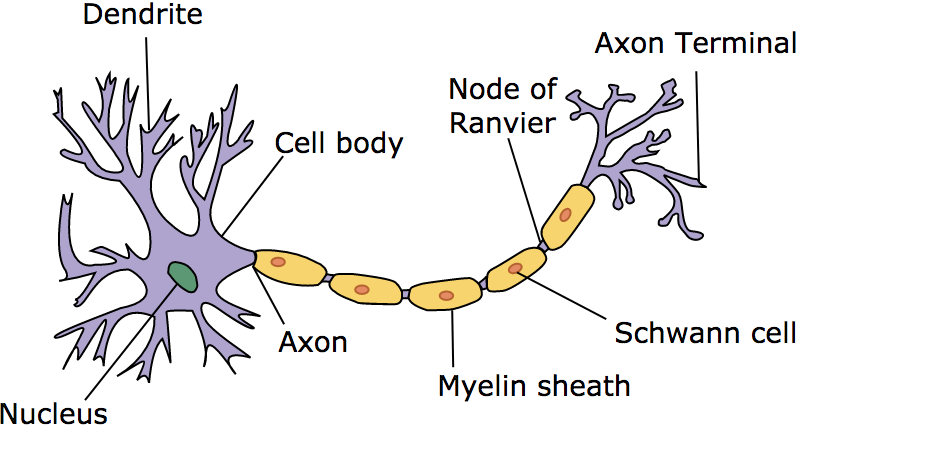
\includegraphics[width=\textwidth]{./images/Neuron.png}
%label the figure so latex can reference it
\caption{Structure of a neuron.\\
Taken from:https://commons.wikimedia.org/w/index.php?curid=1474927}
      \label{fig:Neuron}
\end{figure}


The cell membrane is made up of phospholipids (fat) and separates the cell interior from the extracellular space. The lipid cell membrane is impermeable
to charged ions but thin enough to allow interaction of separated charged
ions through electrostatic forces. Thus the cell membrane acts as an electrical
capacitor. Embedded in the cell membrane are Na$^{+}$ (sodium) and K$^{+}$ (potassium) ion exchange pumps which pump out three Na$^{+}$ ions for every two K$^{+}$ ions pumped in. As a result, Na$^{+}$ is more concentrated outside the cell than inside it, and the intracellular concentration of K$^{+}$ is substantially higher than that outside the cell. There are gated ion channels
(trans-membrane proteins) embedded in the cell membrane which open or close enabling predominantly K$^{+}$, Na$^{+}$, Ca$^{2+}$ (calcium), and Cl$^{-}$ (chloride) ions to flow into and out of the cell. The ion channels act as conductors.

\subsection{Membrane potential}
A potential is a distribution of charge across the cell membrane.
\textit{Voltage} is a measure of the potential energy generated by separated charges and is measured in millivolts (mV). Ions flow into and out of the cell due to both voltage and concentration gradients. \textit{Current} refers to the flow of charged ions into and out of the cell. A resting neuron contains a greater number of negative charges on the inside than on the outside. 
This difference in separated charges is called the neuron's \textit{membrane potential}. A neuron with a membrane potential of approximately -70mV is called \textit{polarized}. This number is also referred to as the resting membrane potential.  

\subsection{Generation of an action potential}
Dendrites contain chemically-gated ion channels, which open when 
a stimulus affects a sensory receptor, such as neurotransmitters binding to the dendrite receptors. As a result, current flows into the intracellular fluid, causing the membrane potential to be less negative or to be positive (depolarization of the neuron). 
This increase in the membrane potential causes the voltage-gated Na$^{+}$ channels, at the entry point of the axon, to open and thus more Na$^{+}$ flows into the cell down its electrochemical  gradient. When a certain threshold is reached ($\approx$ -55mV), an electrical pulse lasting  a short duration ($\approx$ 1ms),  called an \textit{action potential}, is released and is propagated over long distances along the neuron's axon. When the membrane potential rises, the voltage-gated K$^{+}$ channels open, allowing more K$^{+}$ to flow out of the cell, which causes the membrane potential to fall below the resting potential (hyperpolarization of the neuron). The neuron later returns to its resting potential after a refractory period, during which the likelihood of spiking is greatly reduced.


The axon terminal contains voltage-gated Ca$^{2+}$ channels which open causing an influx of Ca$^{2+}$. This leads to the release of neurotransmitters (stored in the synaptic vesicles) into the synaptic cleft. The neurotransmitters then bind to the dendrite receptors of nearby neurons.
A synapse is a specialized structure that facilitates communication between neurons. The neuron that sends off an action potential is called \textit{presynaptic} and the one receiving the chemical message is called a \textit{postsynaptic} neuron. Depending on the chemical properties of the binding neurotransmitters, action potentials fall into two broad categories. Excitatory post synaptic potentials (EPSP) result from excitation of a postsynaptic neuron, while inhibitory post synaptic potentials (IPSP) result from inhibition.

\subsection{Measuring neurons}
The electrical properties of biological cells are measured using electrodes, which allow electrical current to pass through them when they come into contact with electrolytes. Due to the small size of cells, microelectrodes are typically used to measure single unit spiking activity.
A \textit{single unit} refers to a single action potential-generating neuron, whose spikes are clearly isolated by a recording microelectrode \cite{Humphrey1990}.
Neurons are measured using two methods:\textit{extracellular recording} in which an electrode is inserted in the extracellular space near the cell body and  \textit{intracellular recording}, a process where an electrode is inserted inside the cell body (see Figure \ref{fig:Electrodes}).
Intracellular electrodes record membrane potential by comparing the potential on the inserted electrode to that of a reference electrode placed in the extracellular fluid surrounding the cell body. Extracellular recordings can be 
processed (via spike sorting algorithms) to obtain spike times.

\begin{figure}[h]
\centering
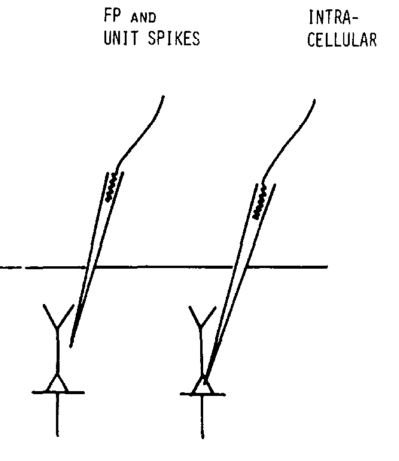
\includegraphics[width=3in]{./images/MeasuringNeuron.png}
\caption{Extracellular (left) and intracellular (right)  recordings, adapted from figure 2 of \cite{Humphrey1990}.}
%label the figure so latex can reference it
      \label{fig:Electrodes}
\end{figure}

Multi-electrode arrays enable simultaneous single-unit recordings from multiple brain sites. The data set we analyze is based on extracellular multiple single-unit single-trial recordings in which spike times of single units have been isolated using suitable spike sorting algorithms.


\subsection{Place cells and place fields}
Place cells are neurons found in the CA1 and CA3 region of the rat hippocampus,
whose firing rate is strongly modulated by the position of the rat within it's
environment. Hence place cells appear to be encoding location \cite{OKeefe1971, OKeefe1978}. The region where a place cell is highly likely to spike is called a place field.

\subsection{Spike trains} 
Experimentalists obtain information that neurons carry about an organism's
environment by measuring from neurons. Spike trains are considered as the 
main mode of information transmission in the nervous system. 
A spike train is an ordered sequence of recorded times at which a neuron
fires an action potential (spike) \cite{Dayan2001}.


\subsection{Raster plot}
A raster plot is a graphical representation of spike trains. In this graph,
a short vertical line is used to show the time at which a spike occurred
in a recorded voltage trace. Figure \ref{fig:RasterPlot}(a) shows a raster plot of real-world data
from the CA1 region of the rat hippocampus. The y-axis represents the neuron
label while the x-axis represents spike times.\\

\begin{figure}[H]
        \centering
        \begin{subfigure}[b]{0.8\textwidth}
            \centering
            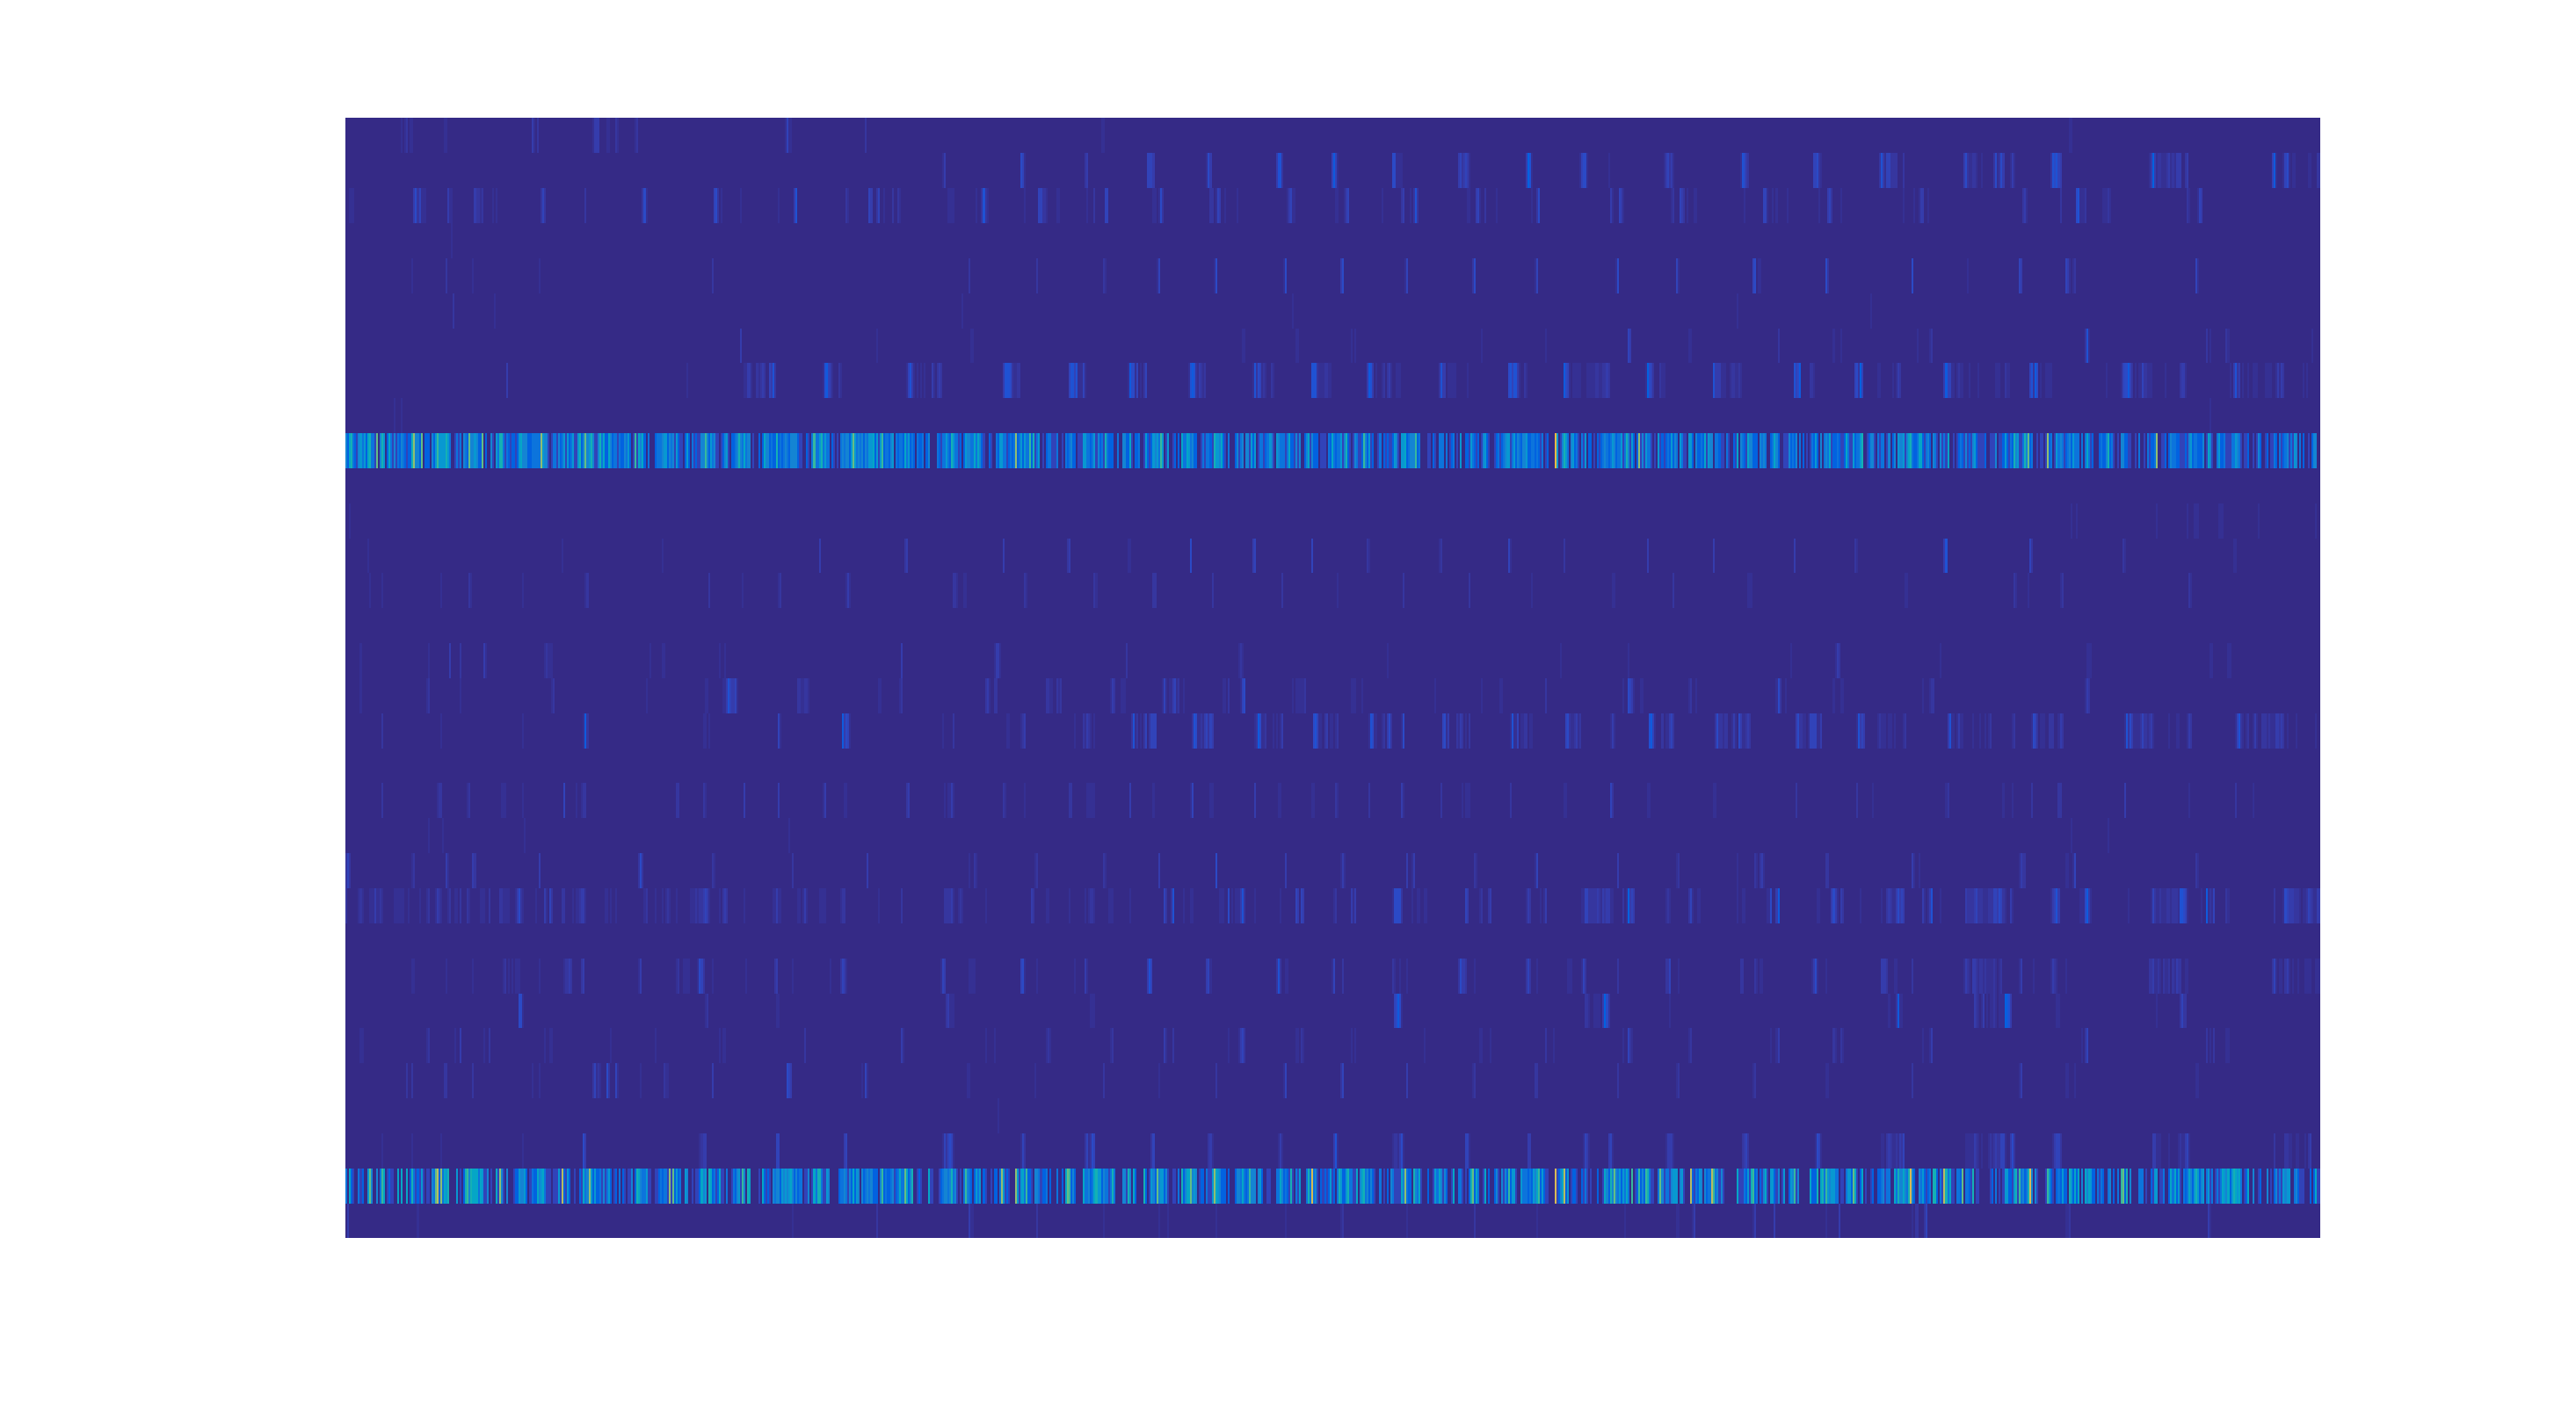
\includegraphics[width=\textwidth]{./images/RasterPlot_large.eps}
            \caption[Raster plot]%
            {{\small Raster plot for 32 neurons from the CA1 region of the rat hippocampus}}    
            \label{fig:Cell activity}
        \end{subfigure}
        
        \vskip\baselineskip
        \begin{subfigure}[b]{0.8\textwidth}   
            \centering 
            \includegraphics[width=\textwidth]{./images/burstNeuronSmall.pdf}
            \caption[]%
            {{\small Firing activity of 32 neurons whose raster plot is shown in (a)}}    
            \label{fig:Prevtime}
        \end{subfigure}
        \caption[Raster plot and bursting neuron]
        {\small Raster plot (a) and firing activity (b) of 32 neurons from the CA1 region of the rat hippocampus based on real-world data provided by the Redish Lab. The data was collected during a behavioral experiment in which the subject was running around a circular maze.} 
        \label{fig:RasterPlot}
  \end{figure}

The goal of our analysis is to investigate the relationship between
spike trains (neural activity) and other variables such as stimuli and location.
It is known that place cell firing is closely correlated with the animal's location in it's environment \cite{OKeefe1971, OKeefe1978, Burgess1994}.



\subsection{Poisson processes}
We represent a spike train as a sequence of random events, that is, as a point process where the random events correspond to spike times. We focus on the simplest point process: a Poisson process, where the numbers of events in non-overlapping intervals are independent random variables. If the probability per unit time (the instantaneous event rate r) is constant, the Poisson process is 
called a \textit{homogeneous Poisson process}. On the other hand if the instantaneous firing rate varies with time, the Poisson process is called a 
\textit{non-homogeneous Poisson process}.



















































%=========================================================================================


%=======Below was my original objective===================================================
%The objective of this present project is to find a low dimensional model of interactions, among a subtype of neurons called place cells, in the CA1 region of the rat hippocampus, believed to be specified to relay the animal's physical position. The model is extrapolated from application of a non-linear dimensionality tool called diffusion maps, to a designed 
%similarity matrix of activity patterns.\\



%======================Gaussian Processes below for future works==============================
%\newpage
%\section{Linear dimensionality reduction techniques}
%\subsection{Gaussian Process Factor analysis}
%\begin{Def}
%A vector-valued random variable $\vect{X} = \left[x_{1}, \ldots , x_{n} \right]^T$
%has a multivariate Gaussian distribution if it's  probability density function is given by
%   
%\[
%f(\vect{x})  = (2\pi)^{-\frac{n}{2}} \det({\Sigma})^{-\frac{1}{2}} 
%\exp \bigg( -\frac{1}{2}(\vect{x - \mu})^{T}\Sigma^{-1}(\vect{x - \mu}) \bigg)
%\]
%
%with mean vector  $\vect{\mu} \in \mathbb{R}^n$ and covariance matrix $\Sigma$.
%The covariance matrix must be a positive semidefinite (PSD) matrix for such a density to exist.
%We write $X  \sim N(\vect{\mu}, \Sigma).$
%
%\end{Def}
%
%
%\begin{Def} A Gaussian Process (GP) is a Gaussian distribution over functions \\
%$f: \mathbb{R}^n \rightarrow   \mathbb{R}^n$  defined by specifying a mean
%function $m: \mathbb{R}^n \rightarrow \mathbb{R}$  and a kernel
%$K: \mathbb{R}^n  \times \mathbb{R}^n \rightarrow \mathbb{R} $ such that the following
%conditions hold:
%
%\begin{itemize}
%\item each vector valued random variable 
%$f(\vect{t}) = \left[f(t_1), \ldots , f(t_n) \right]^T$ has a multivariate Gaussian distribution for all  
%$\vect{t} = \left[t_1, \ldots, t_n   \right]^T$, that is, 
%$f(\vect{t}) \sim  N(m(\vect{t}), K(\vect{t}, \vect{t})).$
%
%\item $m(\vect{t}) = \E(f(\vect{t}))$
%
%\item $K(\vect{t},\vect{s}) = \E\left[ \big(f(\vect{t}) - m(\vect{t}) \big) \big( (f(\vect{s}) - m(\vect{s}) \big)^T   \right]$  for any $\vect{t}, \vect{s} \in \R^n.$  
%
%\item K satisfies the Mercer theorem.
%
%\end{itemize}
%\end{Def}
%
%\begin{Thm}
%
%Every matrix $ K(\vect{t}, \vect{t}) = \{ K(t_i, t_j) \}_{1 \leq i, j \leq n} = (k_{ij}) $
%is a PSD  for all time $\vect{t}$ if
%\[  \vect{v}^T K \vect{v} = 
%\sum_{i=1}^{n} \sum_{j=1}^{n} k_{ij} v_i v_j =
% \sum_{i=1}^{n} \sum_{j=1}^{n} k(t_i, t_j) v_i v_j \geq 0  
% \quad \text{for all}  \quad \vect{v}  \neq \vect{0}. \] 
%
%\end{Thm}
%
%
%\begin{Ex}
%One of the most commonly used kernels is the squared exponential kernel (SE) given by
%$K(t_{i}, t_{j}) = \sigma_{f}^{2} \exp \{-\frac{1}{2l^2}  (t_i - t_j)^2 \}$
%where $\sigma_{f}^{2}$  is the variance of the kernel and l is the length scale.
%
%\end{Ex}
%



%============================================================================================
%%======How to insert a table in latex===================%

%\begin{table}[H]
%   \centering
%    \begin{tabular}{|c|c|c|c|}\hline
%    $x$ & 0 & 1 & 2\\ \hline
%    $f(x)$ & 3 & 6 & 9\\ \hline
%    \end{tabular}
%     \caption{Caption goes here}
%\end{table}

%%=====end table==================================%
%\begin{figure}[H]
%  \centering
%    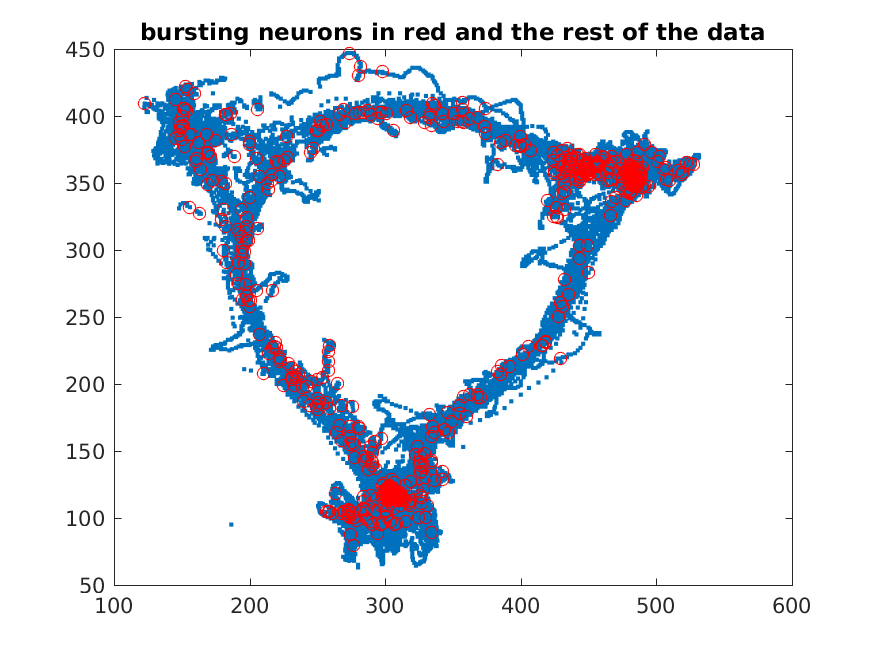
\includegraphics[scale=0.5]{Bursting_neuron.png}
%     \caption{The bursting neuron}
%      \label{tab:data1}
%\end{figure}


%===========Insert a figure in latex=============%






%============end figure===========================%

%\begin{itemize}
%\item What is the nature of the problem you're trying to solve?
%\item Two most well known models that inspired your work
%\item The authors and names of these models
%\item What were they modeling?
%\item Strengths and weaknesses of these models
%\item Overview of our model
%\item What is promising about our model
%\item why are you going to use dimensionality reduction to study the model
%\item why use vector space embeddings instead of the point process framework
%\item Report any results that may be significant and supported by a measure of "goodness"
%\item Mention that this is the first time this type
%of analysis has been applied to the Redish Lab data 
%obtained from the CA1 region of the Hippocampus
%\end{itemize}



\section{Introduction}
 Our perception of the world is influenced by the way our brains processes information received from millions of neurons
 in our nervous system. Even if what we hear, see or feel may vary depending on our environment, information sent to the brain as a result of neural activity consists of a sequence of identical electrical pulses often referred to as spikes.
Thus spike trains are considered as the main mode of information transmission in the nervous system.  Sometimes what neurons encode may be obvious, for instance when a neuron directly responds to a stimulus. However in general,  the way neurons encode information is not known. In this paper, we attempt to answer a central question: how do we understand
and analyze neural responses when the relationship between the way neurons encode information and external variables
such as stimuli, location or behavior  is unclear? 


Our main innovation is  that we  first ignore these external variables and instead look for structure solely within data representing neural activity such as spike trains. Traditional approaches base analyses from the onset on the assumption of a particular relationship between the neural activity and some external variable.
For example, when analyzing the response of visual neurons, one may start out by investigating the dependence of the activity on different visual stimuli. We avoid such apriori assumptions on the relationship between neural responses and any external variable.  Once we have discovered a particular structure in the neural activity, we can then compare the structure
from data to external variables. 


Our primary tool for discovering structure within neural activity data is dimensionality reduction.
Dimensionality reduction considers the problem of  transforming a high-dimensional data set into a new low-dimensional data set in  such a way that preserves as much as possible, the underlying geometry of the data. In our analysis, we use a non-linear dimensionality reduction technique called diffusion maps which finds a low dimensional model of the  data by preserving relative distances between neighboring points on a data manifold. The discovered low-dimensional manifold
can then be related to external variables in order to explore possible relationships between the neural activity and the
external variables.


The  paper is organized as follows: In section 2, we give some biological background on the structure of neurons,
how they are measured and the nature of spikes or electrical signals transferred from neurons to the brain. 
In section 3, we describe some previous work such as classical and modern analyses used to model neural responses
and outline their strengths and weaknesses, if any. In section 4, we give an overview of our current project, simulations and analyses used to model spike time data.  We also introduce a novel method of preprocessing spike time data so as to discover structure in the data. We use dimensionality reduction to analyze our preprocessed data.  In section 5, we report our results on synthetic data as a first step towards analysing real-world spike train data. Our preliminary results on synthetic data show that diffusion maps using spike time data preprocessed by our novel previous time measure,
captures the  one-dimensional manifold corresponding to a simulated rat's movement around a track. In section 6 we give a brief discussion of our results and outline our future directions.
 
 
 
 
 
 
 
 
 
 
 
 
 
 
 
 
 
 
 
 
 
 
 
%Examining stimulus-response data and extrapolating from that a model
%that allows us to predict, given a set of responses, what the stimulus 
%likely was.  Still working on this section.........
%---------This should be more general and give a big picture-------------
%----what do you want to accomplish?
%----what is neural activity in general?
%-----why is a low dim model important?
%-----is idea to understand how the brain is working?
%------How is the brain coding information?
%------how can we decode information based on brain activity?
%----what consequences would there be if we found a low dimensional structure?
%----what is the relevance of having a similarity measure?
%-----e.g want to know whether the brain is thinking about similar things 
%----at different brain states/instances
%----why?  --- what does this have to do with the structure of the space



\section{Biological background}
\subsection{Structure of a neuron}
A neuron is a specialized cell in the nervous system that receives, represents, and transmits information through a series of electrical pulses called action potentials or spikes. The neuron (see Figure \ref{fig:Neuron}) is the fundamental unit of brain function and is made of three major parts: the dendrites (which receive information from other neurons), the cell body or soma (which processes information) and the axon (which transmits information to other neurons) .

\begin{figure}[h]
\centering
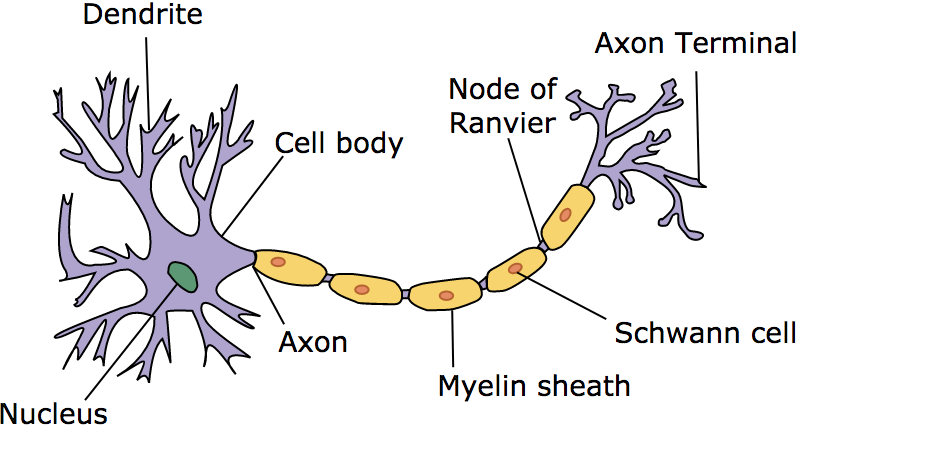
\includegraphics[width=\textwidth]{./images/Neuron.png}
%label the figure so latex can reference it
\caption{Structure of a neuron.\\
Taken from:https://commons.wikimedia.org/w/index.php?curid=1474927}
      \label{fig:Neuron}
\end{figure}


The cell membrane is made up of phospholipids (fat) and separates the cell interior from the extracellular space. The lipid cell membrane is impermeable
to charged ions but thin enough to allow interaction of separated charged
ions through electrostatic forces. Thus the cell membrane acts as an electrical
capacitor. Embedded in the cell membrane are Na$^{+}$ (sodium) and K$^{+}$ (potassium) ion exchange pumps which pump out three Na$^{+}$ ions for every two K$^{+}$ ions pumped in. As a result, Na$^{+}$ is more concentrated outside the cell than inside it, and the intracellular concentration of K$^{+}$ is substantially higher than that outside the cell. There are gated ion channels
(trans-membrane proteins) embedded in the cell membrane which open or close enabling predominantly K$^{+}$, Na$^{+}$, Ca$^{2+}$ (calcium), and Cl$^{-}$ (chloride) ions to flow into and out of the cell. The ion channels act as conductors.

\subsection{Membrane potential}
A potential is a distribution of charge across the cell membrane.
\textit{Voltage} is a measure of the potential energy generated by separated charges and is measured in millivolts (mV). Ions flow into and out of the cell due to both voltage and concentration gradients. \textit{Current} refers to the flow of charged ions into and out of the cell. A resting neuron contains a greater number of negative charges on the inside than on the outside. 
This difference in separated charges is called the neuron's \textit{membrane potential}. A neuron with a membrane potential of approximately -70mV is called \textit{polarized}. This number is also referred to as the resting membrane potential.  

\subsection{Generation of an action potential}
Dendrites contain chemically-gated ion channels, which open when 
a stimulus affects a sensory receptor, such as neurotransmitters binding to the dendrite receptors. As a result, current flows into the intracellular fluid, causing the membrane potential to be less negative or to be positive (depolarization of the neuron). 
This increase in the membrane potential causes the voltage-gated Na$^{+}$ channels, at the entry point of the axon, to open and thus more Na$^{+}$ flows into the cell down its electrochemical  gradient. When a certain threshold is reached ($\approx$ -55mV), an electrical pulse lasting  a short duration ($\approx$ 1ms),  called an \textit{action potential}, is released and is propagated over long distances along the neuron's axon. When the membrane potential rises, the voltage-gated K$^{+}$ channels open, allowing more K$^{+}$ to flow out of the cell, which causes the membrane potential to fall below the resting potential (hyperpolarization of the neuron). The neuron later returns to its resting potential after a refractory period, during which the likelihood of spiking is greatly reduced.


The axon terminal contains voltage-gated Ca$^{2+}$ channels which open causing an influx of Ca$^{2+}$. This leads to the release of neurotransmitters (stored in the synaptic vesicles) into the synaptic cleft. The neurotransmitters then bind to the dendrite receptors of nearby neurons.
A synapse is a specialized structure that facilitates communication between neurons. The neuron that sends off an action potential is called \textit{presynaptic} and the one receiving the chemical message is called a \textit{postsynaptic} neuron. Depending on the chemical properties of the binding neurotransmitters, action potentials fall into two broad categories. Excitatory post synaptic potentials (EPSP) result from excitation of a postsynaptic neuron, while inhibitory post synaptic potentials (IPSP) result from inhibition.

\subsection{Measuring neurons}
The electrical properties of biological cells are measured using electrodes, which allow electrical current to pass through them when they come into contact with electrolytes. Due to the small size of cells, microelectrodes are typically used to measure single unit spiking activity.
A \textit{single unit} refers to a single action potential-generating neuron, whose spikes are clearly isolated by a recording microelectrode \cite{Humphrey1990}.
Neurons are measured using two methods:\textit{extracellular recording} in which an electrode is inserted in the extracellular space near the cell body and  \textit{intracellular recording}, a process where an electrode is inserted inside the cell body (see Figure \ref{fig:Electrodes}).
Intracellular electrodes record membrane potential by comparing the potential on the inserted electrode to that of a reference electrode placed in the extracellular fluid surrounding the cell body. Extracellular recordings can be 
processed (via spike sorting algorithms) to obtain spike times.

\begin{figure}[h]
\centering
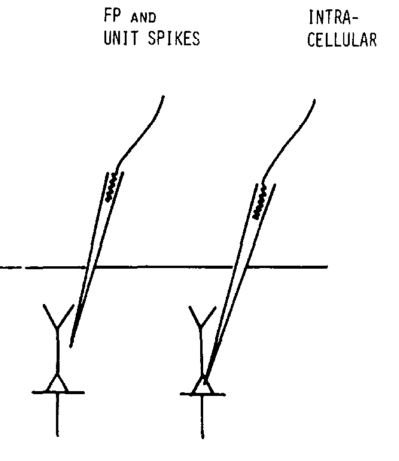
\includegraphics[width=3in]{./images/MeasuringNeuron.png}
\caption{Extracellular (left) and intracellular (right)  recordings, adapted from figure 2 of \cite{Humphrey1990}.}
%label the figure so latex can reference it
      \label{fig:Electrodes}
\end{figure}

Multi-electrode arrays enable simultaneous single-unit recordings from multiple brain sites. The data set we analyze is based on extracellular multiple single-unit single-trial recordings in which spike times of single units have been isolated using suitable spike sorting algorithms.


\subsection{Place cells and place fields}
Place cells are neurons found in the CA1 and CA3 region of the rat hippocampus,
whose firing rate is strongly modulated by the position of the rat within it's
environment. Hence place cells appear to be encoding location \cite{OKeefe1971, OKeefe1978}. The region where a place cell is highly likely to spike is called a place field.

\subsection{Spike trains} 
Experimentalists obtain information that neurons carry about an organism's
environment by measuring from neurons. Spike trains are considered as the 
main mode of information transmission in the nervous system. 
A spike train is an ordered sequence of recorded times at which a neuron
fires an action potential (spike) \cite{Dayan2001}.


\subsection{Raster plot}
A raster plot is a graphical representation of spike trains. In this graph,
a short vertical line is used to show the time at which a spike occurred
in a recorded voltage trace. Figure \ref{fig:RasterPlot}(a) shows a raster plot of real-world data
from the CA1 region of the rat hippocampus. The y-axis represents the neuron
label while the x-axis represents spike times.\\

\begin{figure}[H]
        \centering
        \begin{subfigure}[b]{0.8\textwidth}
            \centering
            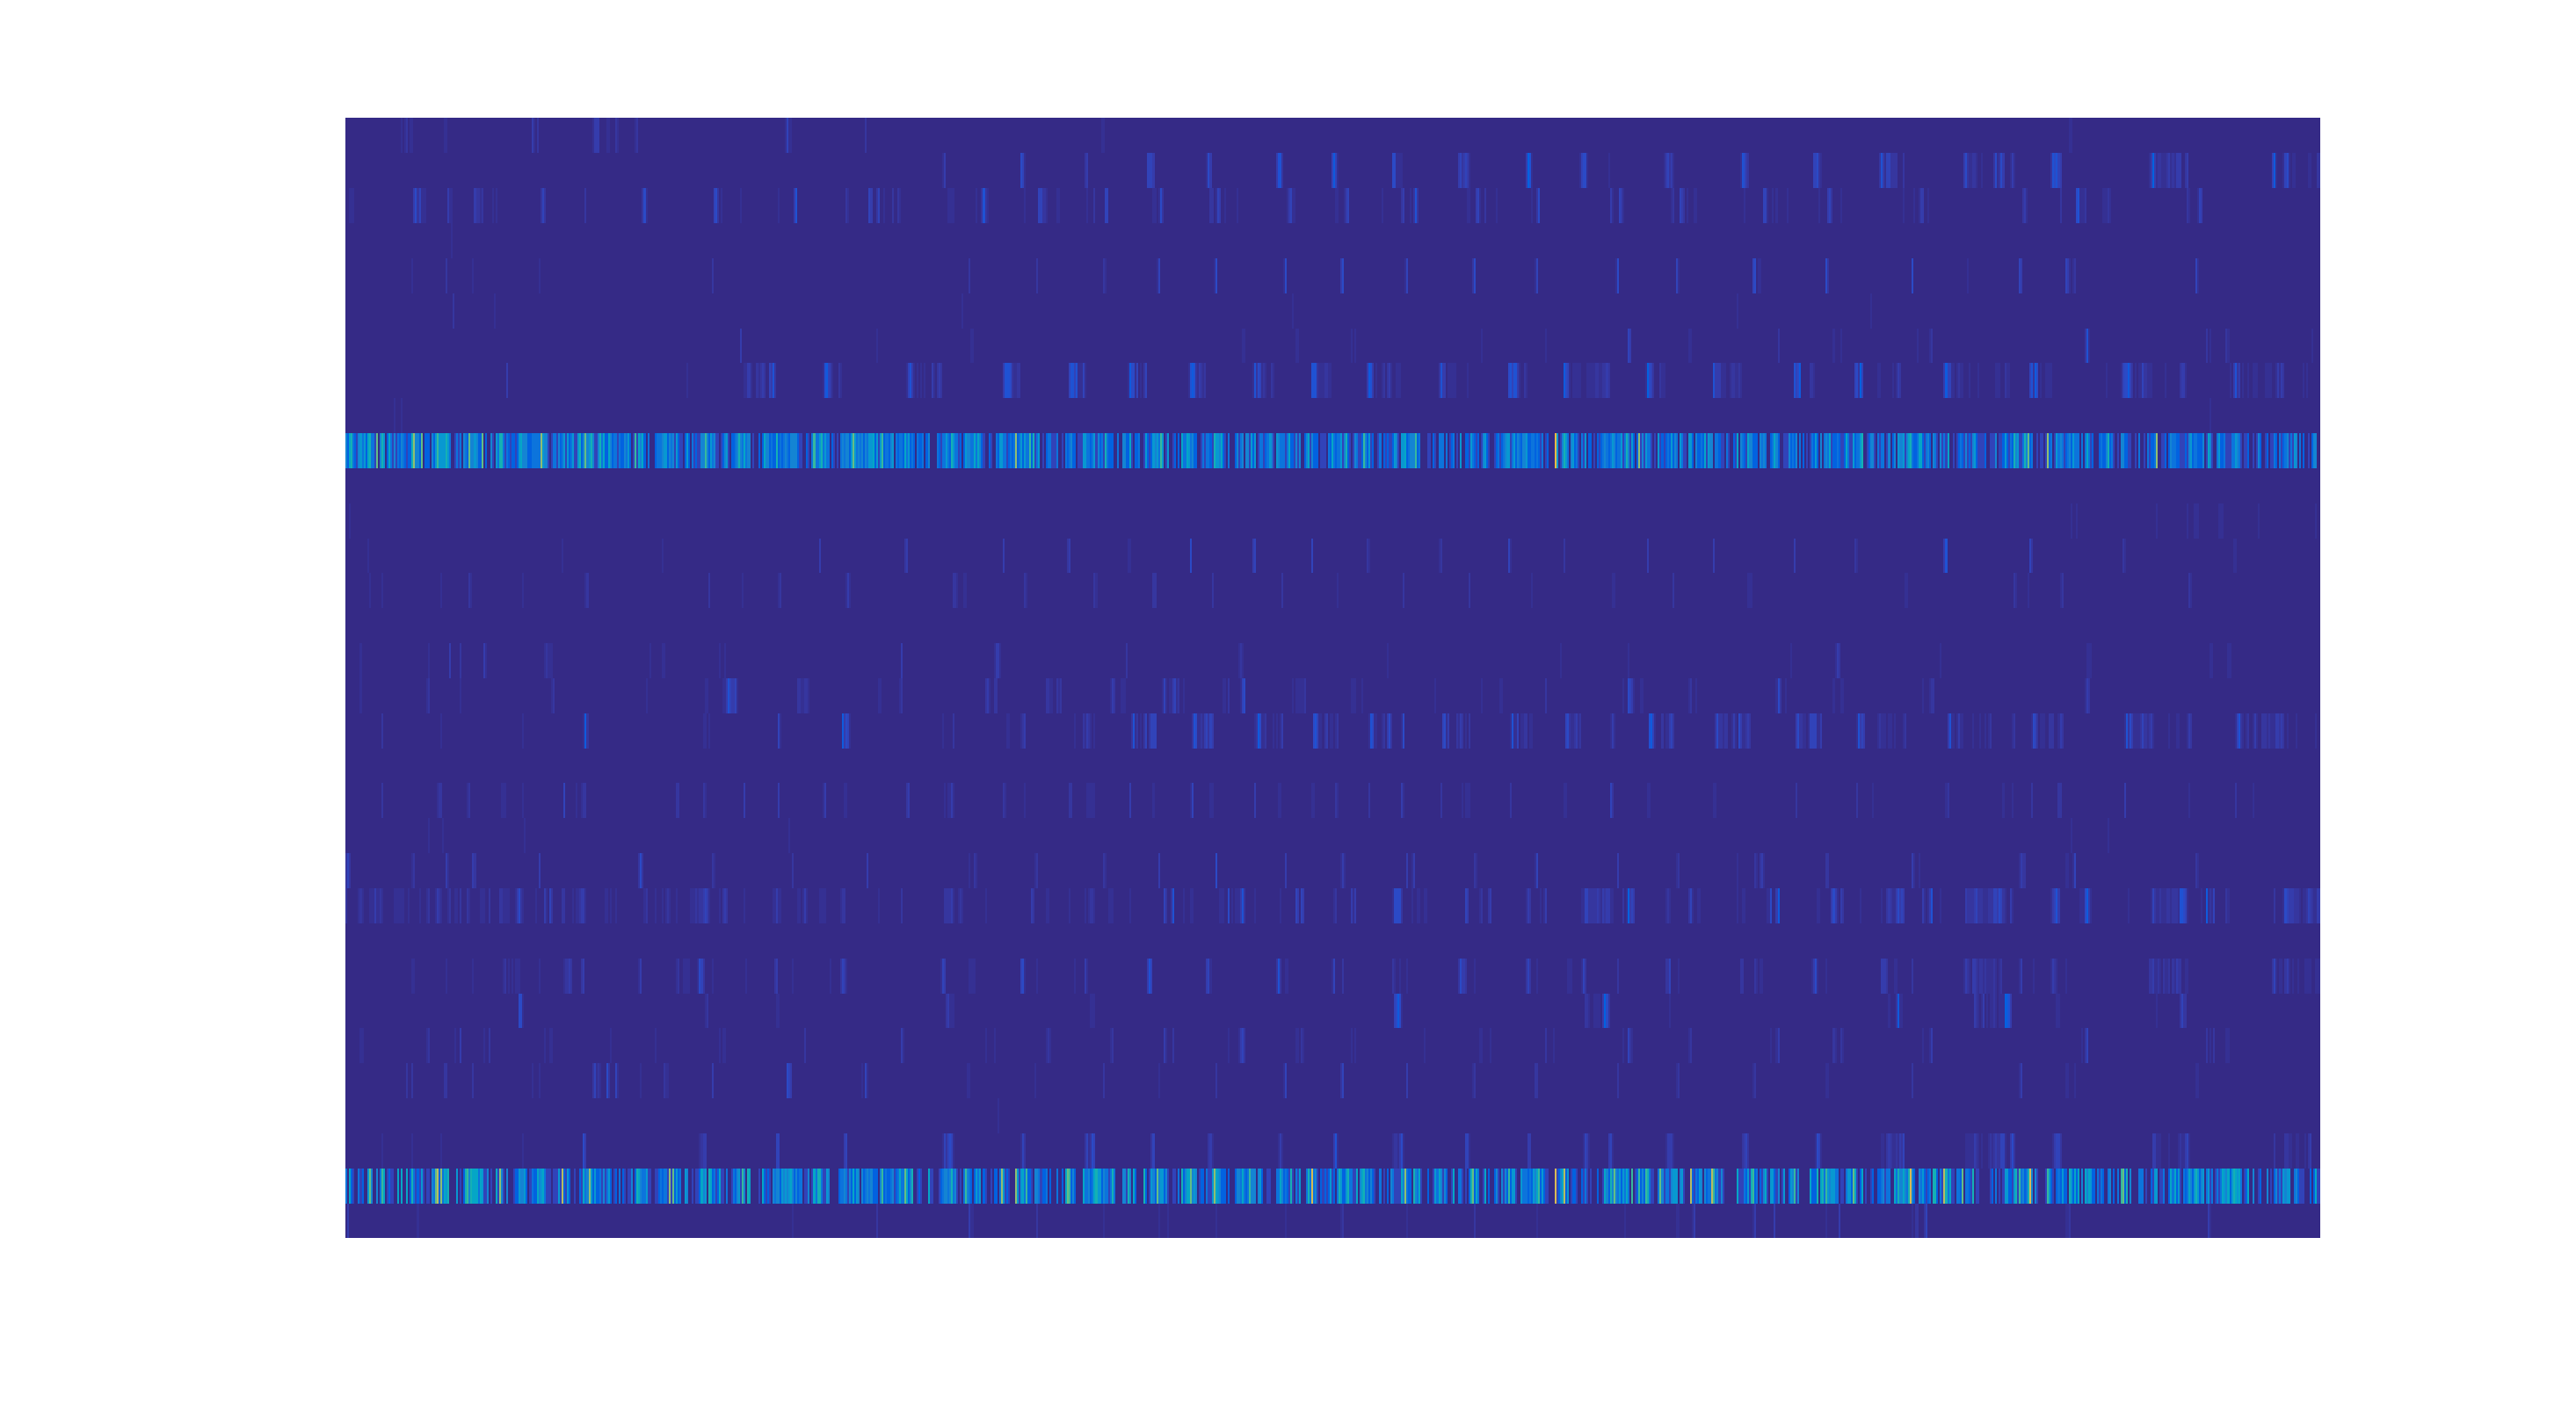
\includegraphics[width=\textwidth]{./images/RasterPlot_large.eps}
            \caption[Raster plot]%
            {{\small Raster plot for 32 neurons from the CA1 region of the rat hippocampus}}    
            \label{fig:Cell activity}
        \end{subfigure}
        
        \vskip\baselineskip
        \begin{subfigure}[b]{0.8\textwidth}   
            \centering 
            \includegraphics[width=\textwidth]{./images/burstNeuronSmall.pdf}
            \caption[]%
            {{\small Firing activity of 32 neurons whose raster plot is shown in (a)}}    
            \label{fig:Prevtime}
        \end{subfigure}
        \caption[Raster plot and bursting neuron]
        {\small Raster plot (a) and firing activity (b) of 32 neurons from the CA1 region of the rat hippocampus based on real-world data provided by the Redish Lab. The data was collected during a behavioral experiment in which the subject was running around a circular maze.} 
        \label{fig:RasterPlot}
  \end{figure}

The goal of our analysis is to investigate the relationship between
spike trains (neural activity) and other variables such as stimuli and location.
It is known that place cell firing is closely correlated with the animal's location in it's environment \cite{OKeefe1971, OKeefe1978, Burgess1994}.



\subsection{Poisson processes}
We represent a spike train as a sequence of random events, that is, as a point process where the random events correspond to spike times. We focus on the simplest point process: a Poisson process, where the numbers of events in non-overlapping intervals are independent random variables. If the probability per unit time (the instantaneous event rate r) is constant, the Poisson process is 
called a \textit{homogeneous Poisson process}. On the other hand if the instantaneous firing rate varies with time, the Poisson process is called a 
\textit{non-homogeneous Poisson process}.



















































%=========================================================================================


%=======Below was my original objective===================================================
%The objective of this present project is to find a low dimensional model of interactions, among a subtype of neurons called place cells, in the CA1 region of the rat hippocampus, believed to be specified to relay the animal's physical position. The model is extrapolated from application of a non-linear dimensionality tool called diffusion maps, to a designed 
%similarity matrix of activity patterns.\\



%======================Gaussian Processes below for future works==============================
%\newpage
%\section{Linear dimensionality reduction techniques}
%\subsection{Gaussian Process Factor analysis}
%\begin{Def}
%A vector-valued random variable $\vect{X} = \left[x_{1}, \ldots , x_{n} \right]^T$
%has a multivariate Gaussian distribution if it's  probability density function is given by
%   
%\[
%f(\vect{x})  = (2\pi)^{-\frac{n}{2}} \det({\Sigma})^{-\frac{1}{2}} 
%\exp \bigg( -\frac{1}{2}(\vect{x - \mu})^{T}\Sigma^{-1}(\vect{x - \mu}) \bigg)
%\]
%
%with mean vector  $\vect{\mu} \in \mathbb{R}^n$ and covariance matrix $\Sigma$.
%The covariance matrix must be a positive semidefinite (PSD) matrix for such a density to exist.
%We write $X  \sim N(\vect{\mu}, \Sigma).$
%
%\end{Def}
%
%
%\begin{Def} A Gaussian Process (GP) is a Gaussian distribution over functions \\
%$f: \mathbb{R}^n \rightarrow   \mathbb{R}^n$  defined by specifying a mean
%function $m: \mathbb{R}^n \rightarrow \mathbb{R}$  and a kernel
%$K: \mathbb{R}^n  \times \mathbb{R}^n \rightarrow \mathbb{R} $ such that the following
%conditions hold:
%
%\begin{itemize}
%\item each vector valued random variable 
%$f(\vect{t}) = \left[f(t_1), \ldots , f(t_n) \right]^T$ has a multivariate Gaussian distribution for all  
%$\vect{t} = \left[t_1, \ldots, t_n   \right]^T$, that is, 
%$f(\vect{t}) \sim  N(m(\vect{t}), K(\vect{t}, \vect{t})).$
%
%\item $m(\vect{t}) = \E(f(\vect{t}))$
%
%\item $K(\vect{t},\vect{s}) = \E\left[ \big(f(\vect{t}) - m(\vect{t}) \big) \big( (f(\vect{s}) - m(\vect{s}) \big)^T   \right]$  for any $\vect{t}, \vect{s} \in \R^n.$  
%
%\item K satisfies the Mercer theorem.
%
%\end{itemize}
%\end{Def}
%
%\begin{Thm}
%
%Every matrix $ K(\vect{t}, \vect{t}) = \{ K(t_i, t_j) \}_{1 \leq i, j \leq n} = (k_{ij}) $
%is a PSD  for all time $\vect{t}$ if
%\[  \vect{v}^T K \vect{v} = 
%\sum_{i=1}^{n} \sum_{j=1}^{n} k_{ij} v_i v_j =
% \sum_{i=1}^{n} \sum_{j=1}^{n} k(t_i, t_j) v_i v_j \geq 0  
% \quad \text{for all}  \quad \vect{v}  \neq \vect{0}. \] 
%
%\end{Thm}
%
%
%\begin{Ex}
%One of the most commonly used kernels is the squared exponential kernel (SE) given by
%$K(t_{i}, t_{j}) = \sigma_{f}^{2} \exp \{-\frac{1}{2l^2}  (t_i - t_j)^2 \}$
%where $\sigma_{f}^{2}$  is the variance of the kernel and l is the length scale.
%
%\end{Ex}
%



%============================================================================================
%%======How to insert a table in latex===================%

%\begin{table}[H]
%   \centering
%    \begin{tabular}{|c|c|c|c|}\hline
%    $x$ & 0 & 1 & 2\\ \hline
%    $f(x)$ & 3 & 6 & 9\\ \hline
%    \end{tabular}
%     \caption{Caption goes here}
%\end{table}

%%=====end table==================================%
%\begin{figure}[H]
%  \centering
%    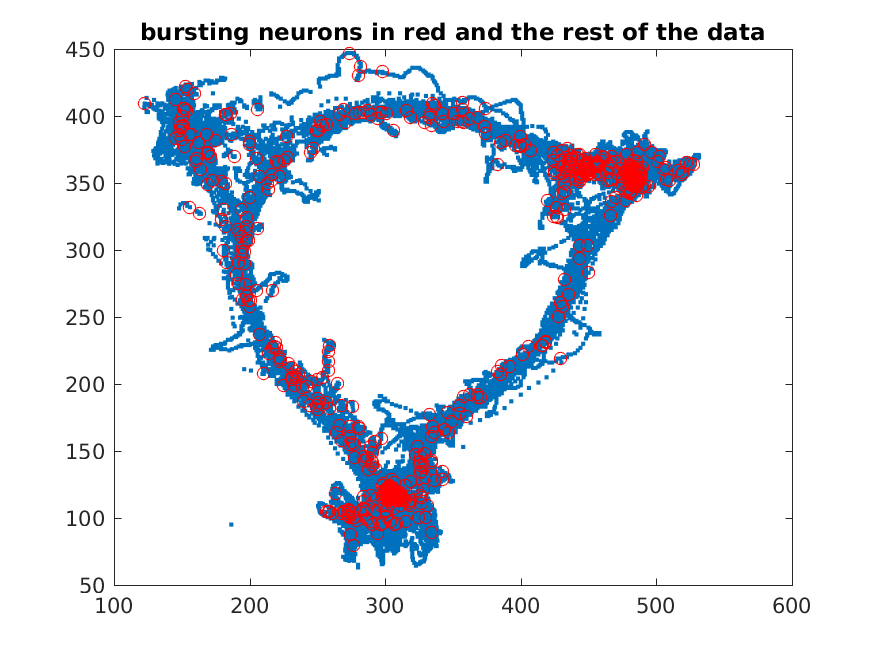
\includegraphics[scale=0.5]{Bursting_neuron.png}
%     \caption{The bursting neuron}
%      \label{tab:data1}
%\end{figure}


%===========Insert a figure in latex=============%






%============end figure===========================%

%\begin{itemize}
%\item What is the nature of the problem you're trying to solve?
%\item Two most well known models that inspired your work
%\item The authors and names of these models
%\item What were they modeling?
%\item Strengths and weaknesses of these models
%\item Overview of our model
%\item What is promising about our model
%\item why are you going to use dimensionality reduction to study the model
%\item why use vector space embeddings instead of the point process framework
%\item Report any results that may be significant and supported by a measure of "goodness"
%\item Mention that this is the first time this type
%of analysis has been applied to the Redish Lab data 
%obtained from the CA1 region of the Hippocampus
%\end{itemize}




%\include{chapters/objectives}
\mychapter{2}{previouswork}

\section{Previous Works}
In this section, we review some previous work based on multi-unit single-trial
and single-trial multiple trial analyses highlighting the strength and
weaknesses of each approach.
We also review some work on spike train analyses based on spike metrics
and their pros and cons.

\subsection{Single-unit multiple trials}

Traditionally, experimentalists developed substantial scientific theories based on analyses from single-unit multiple-trial recordings. For instance, it is known that activity patterns from sensory neurons in the motor cortex of primates are tuned to the direction of the subject's arm movements \cite{Georgopoulos1982}, that neurons in the visual cortex of primates are tuned to the orientation of a stimulus \cite{Hubel1968}, that place cells in the CA1 region of the rat hippocampus are tuned to the animal's position in the environment \cite{OKeefe1971}, in addition to many others.
Classical  methods of analyzing single-unit recordings require averaging of responses across trials in order to estimate the firing rate from which information about the stimulus is decoded. Even though trial averaging may help reduce spiking variability, it does not reduce firing rate (response) variability.
Moreover, the process often results in the smoothing over of rapid fluctuations in the 
responses, which may lead to loss of temporal information in activity patterns, thus yielding incorrect interpretations of the underlying neural mechanisms.
In addition, there are neural mechanisms underlying certain observed phenomena 
that cannot be accounted for using single unit recordings.
For instance, consider that neither sensory neurons tuned to odor \cite{Hopfield1995},
nor certain internal mechanisms such as cognition and decision making (\cite{Redish2016,
Vos2015, Kaufman2014, Mazor2005}, can be controlled by researchers, as can other forms of external stimuli. Such observed phenomena, therefore, can only be analyzed by single-trial multiple-unit recordings. 
\newpage



\subsection{Multiple-unit single trial}

On the other hand however, the use of multi-electrode \cite{Kipke2008} and optical \cite{Kerr2008} recording technologies
has enabled single-trial multiple-unit recording from various brain structures.\\

However, the challenge is that different neurons have highly heterogeneous patterns of activity (neuronal response variability) even on multiple presentation of the same stimulus. Trying to identify all possible activity patterns  corresponding to  a single neuron within the recorded neural population leads to an amplification the number of variables to be considered while modeling collective neural responses. Consequently, biologically motivated assumptions have been made in order to model population activity. For instance, in the dynamical systems perspective, neurons belong to an underlying  tight recurrent connected network within the brain  which may favor correlated responses between neurons \cite{Shenoy2013}.
Among a population of neurons that encode features of a stimulus, the population activity is
correlated with the features of the stimulus \cite{Georgopoulos1982, Hubel1968}.
Thus whether the researcher views the number of stimulus features as lower than the number
of neurons in the population, or views neurons as belonging to an underlying network, it is nonetheless possible to study collective neural activity patterns using a low
dimensional model which captures similar activity patterns among neuronal populations.\\

Lately, dimensionality reduction has been suggested as a tool for modeling population activity. Viewing the recorded N $>1$ neurons as measured variables in the data, dimensionality reduction provides a low dimensional model of the neuronal response space by finding a subset K $<<$ N of directions (dimensions) that explains most of the variability in the neuronal responses. The variability unexplained by the low dimensional model is often regarded as noise \cite{Cunningham2014a}.  Analyses on low dimensional neural population models have been be used to test scientific hypotheses about neural mechanisms that influence a subject's real-world experience. For instance, Mante et al. (2013) used Principle Component Analysis (PCA) and linear regression to show how sensory input is selected and integratedin the prefrontal cortex during decision-making   \cite{Vos2015}.  Kaufman et al. (2014) used Factor Analysis to show evidence of movement preparation before movement in the premotor cortex \cite{Kaufman2014}.  Mazor and Laurent (2005)  used PCA to demonstrate odor discrimination in the olfactory system \cite{Mazor2005}. In the context of exploratory data analysis and visualization, Yu et al. (2009) used Gaussian Process Factor Analysis (GPFA) to characterize single-trial population activity in  macaque premotor and motor cortices during reach planning and execution  \cite{Yu2009} .\\

\subsection{Spike train metrics}
A common approach for quantifying neuronal response variability is through specification of a 
similarity or dissimilarity measure between pairs of spike train data
\cite{Brown2004, Victor1996, Victor1998, Rossum2001,houghton2010measuring, Schreiber2003}.
Here a spike train refers to an increasing sequence of action potentials or spikes
through which the sensory system receives information about the world.
This raises the need for a the notion of ``distance". 
In line with conclusions reached by Victor and Purpura (1996, 1997) and
van Raussum (2001) \cite{Victor1996, Victor1998, Rossum2001}, a short distance between two spike trains approximately represents similar inputs (stimuli) while a large distance between spike trains roughly represents discrimination between different stimuli.
How spike trains encode information is not known. In certain instances, information may be encoded through the precise time at which spikes occur (temporal coding) where as in others, it is encoded through the number of spikes in a given interval (rate coding) (cite Rieke, Warland and Bialek 1996 book on Spikes).
As a remedy for loss of temporal information due to trial averaging, the observation duration is often divided into non-over lapping time intervals called bins.
As long as the size of the bin is larger than the average inter-spike interval (ISI), cross-correlation of binned spike trains provides a good estimate of the instantaneous firing rate
\cite{Brown2004}. The shortcoming of spike binning in studying temporal patterns, is that, two different spike trains often yield identical binning patterns whenever spikes fall in the same bin. Several spike train measures have been designed to overcome the problem of binning. For instance, the edit-length metric \cite{Victor1996, Victor1998} is based on minimizing the cost of transforming one spike train into another by deleting, inserting or shifting a spike. Another measure, the van Rossum distance \cite{Rossum2001, houghton2010measuring} refers to any metric induced on the space of spike trains by transforming a spike train into a continuous function (i.e. a filtered spike train) using a smoothing kernel (such as a box-car window, Gaussian, decaying exponential and  Laplace Kernel) and then using the standard $L^2$ distance on the corresponding function space as the dissimilarity measure. An additional measure, the the correlation-based distance \cite{Schreiber2003} is based on the filtering the spike trains using a Gaussian kernel and then using the normalized dot product between  spike trains as a  similarity measure.
The vector space viewpoint uses van Rossum metrics while the point-process viewpoint
uses metrics such as the edit-length distance \cite{Victor2005}. 
Metrics based on the former often yield  Euclidean distances while those based on the latter are typically non-Euclidean \cite{Aronov2004}.\\



































%\begin{itemize}
%\item what are your long term objectives?
%\item Describe the model you've designed and the metric you're proposing to use
%\item How is this model and metric helping to address short comings of the previous model?
%\item What do you hope to accomplish with this new model?
%\item What new maths theories can be derived from this model?
%\item What are the applications to real world problems
%
%\end{itemize}









%\include{chapters/interpretation}
%\mychapter{4}{Dimensionality Reduction}

\subsection{Dimensionality reduction}\label{spectral decomp}
In this section, we review some linear and non-linear dimensionality reduction techniques. We focus on spectral dimensionality reduction methods where the low dimensional model is obtained from spectral decomposition of an $n \times n$ positive semidefinite (PSD) proximity matrix (see appendices \ref{SVD} and \ref{proximity}). We start by defining dimensionality reduction and outline steps of spectral dimensionality reduction. Next, we give a brief description of PCA and the diffusion maps algorithm for dimensionality reduction. In later sections, we compare the performance of PCA and diffusion maps on our spike train data set.


\subsubsection{Overview of spectral dimensionality reduction}
Let $\textbf{X} = \displaystyle \{\vect{x}_{1}, \ldots , \vect{x}_{n} \}$
be a set of $n$ data points, each of which is associated with $N$ features, so that each $\vect{x}_{i}$ is a point in a high dimensional space $\R^{N}$. For convenience, we often view the set of data points $\Bm{X}$ as a matrix, $\Bm{X} \in \mathbb{R}^{n \times N}$.
Assume that the data points lie on or near an underlying $l$-dimensional manifold embedded in the high dimensional space where $l$ is much smaller than $N$. Dimensionality reduction considers the problem of  transforming the high dimensional data set $\textbf{X}$ into a new data set $\textbf{Y} = \displaystyle \{ \vect{y}_{1}, \ldots, \vect{y}_{n} \}$  of $n$ points, each of which is associated
with a smaller set of $l$ features, which are possibly new or a combination of the original $N$ features, and such that each $\vect{y}_{i} \in \R^{l}$ is a low dimensional representation of $\vect{x}_{i} \in \R^{N}$. In addition the transformation must preserve, as much as possible, the underlying geometry of the data.\\

Spectral dimensionality reduction (SDR) refers to all dimensionality reduction methods which obtain a low dimensional model of $\Bm{X}$ by carrying out four main steps \cite{Lawrence2010}.
\begin{itemize}
\item[i)] A distance $b_{ij} = \text{dist}(\vect{x}_{i}, \vect{x}_{j})$, between data points
is chosen and a real number $l, 1 \leq l < N$ representing the desired dimensionality is fixed.
\item[ii)] From the distance, an $n \times n$ PSD proximity matrix  is computed (see appendix \ref{proximity}).
\item[iii)] Spectral decomposition is carried out on the generated PSD matrix and
the top $l$ eigenvectors $\{ \vect{v}_{1}, \ldots, \vect{v}_{l} \}$ of the proximity matrix
form the columns in a new matrix, $\Bm{V} = [\vect{v}_{1}, \ldots, \vect{v}_{l}] \in \R^{n \times l}.$
\item[iv)] Viewing the $i^{th}$ row of $\Bm{V}$ as a point $\vect{y}_{i}$
in $\R^{l}$, a new set of $n$ points 
$\{\vect{y}_{1}, \ldots, \vect{y}_{n} \}$ is obtained such that each
 $\vect{y}_{i} = (\vect{v}_{1}(i), \ldots, \vect{v}_{l}(i)) \in \R^{l}$
is a low dimensional representation of $\vect{x}_{i} \in \R^{N}$.
\end{itemize}


\subsubsection{Linear dimensionality reduction}
Let $\Bm{X} \in \R^{n \times N}$ be a matrix of $n$ data points in a high dimensional space $\R^{N}$. Linear dimensionality reduction refers to the problem of finding a low dimensional model using a linear transformation of the data. The low dimensional model of the data $\Bm{Y}$, is obtained using the relation $\Bm{Y} = \Bm{M}^{\top}\Bm{X}$ where $M$ is an $n \times l$ matrix with $l \ll N$. A common spectral linear approach is principle component analysis (PCA) \cite{JolliffeIT1986PCAa}. PCA is a linear technique for finding the directions of maximum variance in the data. The main assumption in PCA is that the high dimensional data lie on or near a low $l$-dimensional linear subspace embedded in some high dimensional space $\R^{N}$. 
The low dimensional model that describes the data is found via spectral decomposition of the sample covariance matrix as follows:

\begin{itemize}
\item[i)] Let $\textbf{X}$ be the centered data formed by subtracting the mean from each point.
\item[ii)] Summarize the correlation relationships between the zero-mean data points by computing the sample covariance matrix $\frac{1}{n}\textbf{XX}^{\top}.$
\item[iii)] Find the spectral decomposition of $\textbf{XX}^{\top}$ or 
use SVD to find $\textbf{X} = \bm{U\Sigma V^{\top}}$  (see appendix \ref{SVD}).
\item[iv)] Let $\bm{V}_{l}$ denote the top $l$ columns of $\textbf{V}$ corresponding to the  top $l$ singular values of $\textbf{X}$.
\item[v)] The low dimensional model $\textbf{Y}$ is obtained by setting 
$\textbf{Y} = \textbf{V}^{\top}\textbf{X}$.
\end{itemize}

\subsubsection{Non-linear dimensionality reduction}

Methods like PCA assume that the underlying manifold on which the data lie is globally linear. This implies that the shortest distance between any two points while traveling along the data manifold is a straight line.
However, any dimensionality reduction technique must preserve the underlying geometry of the data manifold. In particular, points that are close together in the high dimensional space should be mapped closer to each other in the low dimensional space where as points that are far apart in the high dimensional space must remain far apart in the embedded space. In particular, we ignore long distances in the embedded space. This idea of preserving relative distances between points
in both the input space and embedded space is based on the multidimensional scaling (MDS) approach.
Figure \ref{fig:Swiss roll} illustrates the limitations of linear techniques on highly curved manifolds like the swiss roll and helps to highlight the importance of non-linear dimensionality reduction techniques.

\begin{figure}[h]
\centering
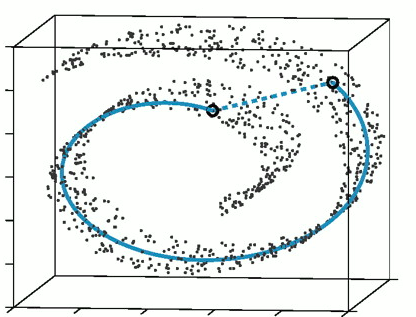
\includegraphics[width=3.5in]{/home/tesylvia/Oral_Sept_2017/images/ISOMAP.png}
%label the figure so latex can reference it
\caption{For a linear method like PCA, the two circled points on the swiss roll would be close together even though they are far apart when using geodesic distances. Taken from \cite{TenenbaumJB2000Aggf}.}
      \label{fig:Swiss roll}
\end{figure}


\subsubsection{Multidimensional scaling (MDS)}
Assume that an $n\times n$ matrix, $\Bm{B}$=(b$_{ij}$), of pair-wise distances
(not necessarily Euclidean) or similarities (see appendix \ref{proximity}), $\Bm{S} = (s_{ij})$, between data points, $\{\vect{x}_{1}, \ldots, \vect{x}_{n} \}$, is given and $n$ is large.
Multidimensional scaling (MDS) \cite{CoxT2000, MardiaK.V1979Ma} considers the the problem of finding a low dimensional model of the high dimensional data by searching for a configuration of $n$ points $\{\vect{y}_{1}, \ldots, \vect{y}_{n} \}$ in $\R^{\text{l}}, \text{l} \ll \text{n}$, where each $\vect{y}_{i}$ is a low dimensional representation of $\vect{x}_{i}$, and such that relative pair-wise distances between points are preserved. Specifically, the Euclidean distances between the configuration points, $\norm{\vect{y}_{i} - \vect{y}_{j}}_{2}$, must be as ``close" as possible to  the given distances, b$_{ij}$, that is, $\norm{\vect{y}_{i} - \vect{y}_{j}}_{2} \approx \text{b}_{ij}$, for all $1 \leq i, j \leq n$.

\subsubsection{Spectral non-linear dimensionality reduction}
Spectral non-linear dimensionality reduction (SNLDR) techniques are a 
class of MDS methods which find a low dimensional model of the data by preserving relative distances between neighboring points on a data manifold. These are the non-linear dimensionality
reduction algorithms that we will consider. Examples of SNLDR methods include ISOMAP \cite{TenenbaumJB2000Aggf}, locally linear embedding (LLE)  \cite{roweis2000nonlinear}, Laplacian eigenmaps (LE) \cite{belkin2003laplacian} and diffusion maps \cite{coifman2006diffusion}, in addition to many others. Unlike linear dimensionality reduction techniques, SNLDR methods do not make apriori assumptions about the underlying geometry of the data manifold.
SNLDR methods model local neighborhood relations between data points by building a graph on the data  \cite{Luxburg2007}. We only review the diffusion maps algorithm.


\subsubsection{Key graph theory concepts}
The non-linear dimensionality reduction algorithms we consider are based on graph theory. Hence, we first introduce three key graph theory concepts that we need: a weighted undirected graph, the degree matrix and the graph Laplacian.\\

A graph is a tuple $G = (V,E)$ where $V = \{v_1, \ldots , v_n\}$ is a finite set of points called vertices or nodes and $E$ is a finite collection of edges connecting pairs of vertices. The graph $G$, is undirected if the edges between vertices are bidirectional.
We can make a weighted graph by assigning a weight or number $w_{ij}$, to an edge $e_{ij} \in E$, between a pair of vertices $(v_i, v_j) \in V$. A connectivity matrix or similarity matrix $\Bm{W}$, of $G$, is the matrix whose $(i,j)$-th entries are edge weights $w_{ij}$.
The degree $d_i$, is the sum of weights $w_{ij}$, of all edges connected to a vertex $v_i \in V$.
A diagonal matrix $\Bm{D}$, with degrees, $d_{i}$, on its diagonal is called the degree matrix.
The unnormalized graph Laplacian is the  matrix $\Bm{L = D} - \Bm{W}$.


\subsubsection{Neighborhood graph}
We can approximate small distances between points in the input space using the usual Euclidean distance between nearby points in the embedded space as in linear approaches. However, long distances in the input space are not necessarily equal to long distances in the feature space (see figure \ref{fig:Swiss roll}). One way to address this problem is to ignore long distances in the embedded space by building a graph $G = (V, E)$ on the data. We ignore long distances by placing an edge $e_{ij} \in E$ only between neighboring vertices $(v_i, v_j) \in V$. The result is called 
a neighborhood graph.\\

A particular type of neighborhood graph is the $\epsilon-$neighborhood graph constructed as follows. Suppose we are given a data set, $\Bm{X} =  \{\vect{x}_{1}, \ldots, \vect{x}_{n} \}$ and assume that the pairwise distances, $b_{ij} = \text{dist}(\vect{x}_{i}, \vect{x}_{j})$, between points are known. Identifying each data point with a vertex $v_{i} \in V$, on a graph $G = (V, E)$, we can build a weighted  undirected graph on the data by placing an edge $e_{ij} \in E$, between vertices $(v_i, v_j) \in V$, if $x_i$ and $x_j$ are sufficiently close. We weight the edge $e_{ij} \in E$, by a similarity measure $s_{ij}$, derived from the given distances (see appendix \ref{proximity}). The resulting $\epsilon-$nearest neighborhood graph represents the local distances among points.\\

For diffusion maps, the neighborhood graph is modified to a fully connected graph, but where the weights are approximately zero whenever the distance between data points is large.
To do this, we use a similarity function that captures local neighborhood relations between points and at the same time decays to zero so fast that we do not have to truncate the weights. In particular, in diffusion maps, we use the similarity function 
$w_{ij} = e^{- \frac{\text{dist}^{2}(\vect{x}_i, \vect{x}_j)}{2 \sigma^2}}$. 
In this way, $\sigma$ plays the role of $\epsilon$, in that it specifies the width of the neighborhood.

\subsubsection{Basic idea of the diffusion maps algorithm}
The diffusion maps algorithm consists of several steps which are outlined in appendix \ref{diffusion maps}. Below is a brief summary of the diffusion maps algorithm.

\begin{itemize}
\item[1)] Given the pairwise distance dist$(\vect{x}_i, \vect{x}_j)$, compute the weight matrix 
$\Bm{W} = (w_{ij})$, between data points by setting
$w_{ij} = \displaystyle e^{- \frac{\text{dist}^{2}(\vect{x}_i, \vect{x}_j)}{2 \sigma^2}}$.
\item[2)] Let $d_{i} = \sum_{j = 1}^{n} w_{ij}$ be the degree of the $i^{th}$ node and compute the degree matrix $\Bm{D} = \text{diag}(d_{1}, \ldots, d_{n})$.
\item[3)] Define a random walk on the graph of the data (see appendix \ref{random walk}) by specifying $p_{ij} = \displaystyle \frac{w_{ij}}{d_{i}}$, the probability of going from vertex $v_i$ to $v_j$ in one-step. Organize the pair-wise transition probabilities in an $n \times n$ 
transition probability matrix $\Bm{P} = \Bm{D}^{-1}\Bm{W}$ with $\Bm{P} = (p_{ij})$.
\item[4)] Normalize $\Bm{P}$ to obtain a PSD similarity matrix $\Bm{S}$ given by
$\Bm{S} = \Bm{D}^{\frac{1}{2}}\Bm{P}\Bm{D}^{\frac{-1}{2}}$.
\item[5)] Compute the SVD of $\Bm{S}$ and write $\Bm{S} = \Bm{V}\bm{\Sigma}\bm{V^{\top}}$ where,
$\bm{\Sigma} = \text{diag}(\lambda_{0}, \ldots, \lambda_{n-1})$ with ordered eigenvalues, 
$\lambda_{0}\geq \lambda_{1} \geq \ldots \geq \lambda_{n-1}$ and corresponding eigen vectors 
$\Bm{V} = [v_0, v_1 \ldots, v_{n-1}]$.
\item[6)] The l-dimensional embedding of the $i^{th}$ data point $\vect{x}_i$
in the low dimensional space $\mathbb{R}^{l}$ is the map
$$ \vect{x}_{i} \mapsto  \begin{bmatrix}
         \lambda_{1}^{t}\phi_{1}(i)\\
         \lambda_{2}^{t}\phi_{2}(i)\\
         \vdots\\
         \lambda_{l}^{t}\phi_{l}(i)
        \end{bmatrix} .$$
where $\{ \phi_{0}, \phi_{1}, \ldots, \phi_{n-1} \}$ are the right singular vectors of $\Bm{P}$
and $\lambda_{i}^{t}$, are obtained from the t-step transition probability matrix $\Bm{P}^{t}$
(see appendix \ref{diffusion maps}).
\end{itemize}































%%%%%%%%%%%%%%%%%%%%%%%%%%%%%%%%%%%%%%%%%%%%%%%%%%%%%%%%%%%%%%%%%%%%%%%%%%%%%%%%%%%%%%%%%%%
%%%%%%%%%%%%%%Laplacian Eigen Maps algorithm %%%%%%%%%%%%%%%%%%%%%%%%%%%%%%%%%%%%%%%%%%%%%%
%\subsubsection{Laplacian eigen maps algorithm}
%Building a Graph from a data set $X = \{\vec{x}_{1}, \ldots , \vec{x}_{n}\}$}
%\pause
%Assuming the pairwise distances $d_{ij}$ or similarities $s_{ij}$ between data points $\{x_{1}, \ldots, x_{n}\}$
%are known, the points may be connected using 
%
%mutual k-nearest neighbor graph
%
%
%Build a weighted graph on the given data set
%by viewing data points as vertices of a graph in which neighboring points are connected by weighted edges
%
%From the adjacency matrix W  using one of the two methods
%
%Choose the weights $w_{ij}$ using the Heat Kernel with no parameter
%\[
% w_{ij} =
%  \begin{cases} 
%      \hfill e^{-\frac{\norm{\vec{x}_{i}-\vec{x}_{j}}^2}{t}}    \hfill & \text{ if $(i,j) \in E$} \\
%      \hfill 0 \hfill & \text{otherwise} \\
%  \end{cases}
%\]
%\pause
%
%\item Case 2: (No Parameter t).
%
%\[
% w_{ij} =
%  \begin{cases} 
%      \hfill 1    \hfill & \text{ if $(i,j) \in E$} \\
%      \hfill 0 \hfill & \text{otherwise} \\
%  \end{cases}
%\]
%
%
%
%
%
%and degree matrix D,
%compute the graph Laplacian L using the relationship L = D-W
%
%Solve the generalized eigenvalue problem Lv = $\lambda$Dv
%and stack the smallest  eigenvectors $\{\vec{v}_{1}, \ldots, \vec{v}_{d} \}$ of L excluding the smallest eigenevector of L as columns in a matrix U ;
%obtain a d-dimensional embedding of the data
% by viewing each  data point as the $i^{th}$ row of U via the map
%$\vec{x}_{i} \mapsto (\vec{v}_{1}(i), \ldots, \vec{v}_{d}(i))$ };
%
%
%
%
%
%
%\item Solve the generalized eigenvalue problem $L\vect{v} = \lambda D \vect{v}$ and take the bottom d-smallest generalized eigenvectors $\vect{f}_{2}, \ldots, \vect{f}_{d}$ of L excluding the constant eigenvector.
% \pause
% \item Form the matrix U = $[\vect{f}_{2} \ldots \vect{f}_{d}]$ by stacking $\vect{f}_{i}$ as columns in U.
% \pause 
% \item View the $\text{i}^{th}$ row of U as the $d$-dimensional representation of the $\text{i}^{th}$ vertex 
% corresponding to the original data point $\vect{x}_{i}.$
%






























%\include{chapters/nextsteps}
%\mychapter{3}{methodology}

\section{Current Project}

\subsection{Our framework}

We propose a novel method of pre-processing spike times by looking at the time since the previous spike, which we refer to as the previous time.  Currently, our pre-processing technique is  applied to synthetic data as a first step towards being
able to pre-process  real-world data using the previous time.  To the best of our knowledge, using previous time  to pre-process spike train data from the CA1 region of the rat hippocampus has never been done before.\\

Our preliminary results on synthetic experiments  show  that  previous time data  capture  the  four and a half laps taken by a rat  around a simulated circular track.  We use the diffusion maps algorithm \cite{coifman2006diffusion}  to obtain a low dimensional model of the simulated data and compare the algorithm's performance with that of PCA.\\

Traditionally, spike trains are often smoothed using a suitable kernel (see section 3.4.2) in order to obtain an estimate
of the  firing rate.  Smoothing a simulated firing rate with a kernel such as a Gaussian or decaying exponential  and then adding additive and Poisson noise to the simulated firing rate could be an ideal way to generate synthetic data which closely mimics the nature of the real-world  data we have. However  there are many parameters to tune when using kernels.
Moreover,  we do not have  a suitable measure of error for  analyzing the performance  of the diffusion maps  algorithm and PCA on our synthetic data. To work around these two obstacles, we simulate clean firing rate data which perfectly encodes the position of the animal on a circular track and compare the output of the  two algorithms on both the clean firing rate data and the noisy previous time data. \\

Our motivation for using both  firing rate data  and previous time data  is based on the fact that the position of the rat is coded by place cells using both the firing rate and the precise time at which the cells fire with respect to the hippocampal theta rhythm. The theta rhythm is a sinusoid of frequency 7-12 Hz which occurs whenever a rat changes position in  a specific direction \cite{OKeefe1971, Burgess1993}.\\


In section  4.2 and 4.3,  we define the previous time function and illustrate it graphically.  In addition, we give a description of our simulation and analyzes used. In section 5, we show our results of diffusion maps and PCA on synthetic data sets.
Finally in section 6, we give a brief discussion on our results and suggest possible future directions.


\subsection{Nature of our raw real-world data}
The  raw real-world data set consists  of multiple single-unit single-trial spike trains,\\
\[ 
\text{T}^{\text{spike}} = \displaystyle \{ \{ t^{j} \} ,  1 \leq j \leq 32 \}  
\]
recorded from 32 neurons, called  place cells, in the CA1 region of the rat hippocampus, where,
$\displaystyle  \{t^{j}\} =  \{t_{1}^{j}, ....., t_{n_{i}}^{j} \} $, represents  a sequences of n$_{i}$ recorded times at which the spikes of the $j^{th}$ neuron occurred. \\
However, we only show results based on synthetic data due to lack of a suitable measure of error to quantify 
the performance of  diffusion maps and PCA on real world data.  We pre-process the simulated spike trains by computing  the previous time  defined in section 4.3.
 

%%%%%%% %%%  deleted this because our firing rate does not have spikes   %%%%%%%%%%%%%%%%%%%%%%%%%%
%\subsubsection{Conversation to a firing rate}
%For each neuron labeled $j$,  we smooth the corresponding spike train T$^{\text{spike}}_{j}(t)$ to obtain the firing rate function $R^{j}(t).$ The  firing rate function, for the $j^{th}$ neuron is given by
%\begin{equation} \label{jfirerate}
%\text{R}^{j}(t) = \displaystyle \sum_{i=1}^{n_{i}}  \frac{1}{\sigma \sqrt{2\pi}} 
%e^{-\dfrac{(t_{i_{k}}^{j}  - t_{i_{l}}^{j})^2}{2\sigma^2}}. 
%\end{equation}
%%%%%%%%%%%%%%%%%%%%%%%%%%%%%%%%%%%%%%%%%%%%%%%%%%%%%%%%%%%%%%%%%%%%%%%%

\subsection{The previous time function}

Given any time $t$, define the previous time function of the $j^{th}$ neuron, denoted by $\text{P}^{j}(t)$ as follows. Let 
\[
t^{j}_{\text{prev}}(t) = \displaystyle \max  \{  t^{j}_{i} \ \ | \ \ t^{j}_{i} < t, 1 \leq i \leq n_{i} \} \ \ \text{for all spike trains} \quad  \{t^{j}\} \in T^{\text{spike}}, 
\]
where $t^j_i$ denotes the $i^{th}$ spike of the $j^{th}$ neuron.  The previous time function, P$^{j}(t)$, is given by, 
\begin{equation}\label{prevtimefun}
\text{P}^{j}(t) = t^{j}_{\text{prev}}(t) - t.
\end{equation}
Previous time refers to the time since the last spike of a given neuron. The previous time function captures the history of the neuron's  activity even in the absence of spikes.

Figure \ref{fig:PrevTime} below illustrates how the previous time function is obtained from the firing activity of a given neuron.


 \begin{figure}[H]
        \centering
          \includegraphics[width=\textwidth]{./images/PrevTime_graph.pdf}
           \caption[]
            {\small The previous time function $\text{P}^{j}(t) = t^{j}_{\text{prev}}(t) - t,$ based on a raster plot of a single neuron.   $P^{j}(t)$ is equal to zero when a neuron fires a spike  and then moves away from zero with a slope of negative one to a height equal to the difference between two adjacent spike times, below the horizontal axis. } 
             \label{fig:PrevTime}
  \end{figure}


\subsection{Simulation}
We consider a population of $N=32$ sensory neurons (place cells) encoding a 
one-dimensional circular stimulus variable, $\theta(t)$, which represents 
the position of a rat, at any time $t$ along a circular track, during a behavioral task.
We let $\theta(t) = c t \ \ (\text{mod} \ \ 2\pi)$, where time $t$, is in seconds, $c = \dfrac{2\pi}{T_{\text{lap}}}$ is the speed of the animal, and
$\text{T}_{\text{lap}}$ is the time taken for the animal to make one lap around the circle.
From  $\theta(t)$,  we model the place field of the $j^{th}$ neuron using a Gaussian 

\begin{equation}
{g}^{j}(\theta) = \displaystyle  f_{\text{bg}} + f_{\max} 
\exp\bigg(-\dfrac{\text{dist}^{2}(\theta - \phi_{j})}{2\epsilon_{j}^{2}} \bigg)
\end{equation}

where $f_{bg}$ is the background firing rate that is independent of the underlying stimulus, $f_{\max}$ denotes the maximum firing rate of each neuron, $\epsilon_j \in  [0.01, 1]$ is the width of the $j^{th}$ neuron's place field  and $\phi_{j}$ is the preferred position of the $j^{th}$  neuron or the center of the j$^{th}$ place field. We assume that the centers of the place fields are distributed uniformly in space.  In particular, we set 
$$\phi_j = \frac{j2\pi}{N}, \ \    \text{for}   \ \    1 \leq j \leq N.$$
Intuitively, $g^{j}(\theta)$, models  the likelihood that the rat's neuron fires given the animal's position $\theta(t)$, in space.
The Gaussian function indicates that the rat's place cell is  likely to fire maximally  at the center of the cell's place field
which mimics a characteristic  of a real-world rat's place cells.
Our model assumes that each neuron in the simulated rat's brain has a single place field. This is a realistic assumption as 
most place cells have one place field (see section 6 on possible future directions). \\

Given any two angles, $\theta_{1}, \theta_{2} \in [0, 2\pi]$, the quantity
$\text{dist}(\theta_{1}, \theta_{2})$ denotes the shortest distance between 
two points on a unit circle, given by
\[
\text{dist}(\theta_{1}, \theta_{2}) = \abs{\big( \big( (\theta_{1} - \theta_{2}) + \pi  \big) \ \ \text{mod} \ \ 2\pi \big) - \pi}.
\]

Our simulation assumes  that information about the animal's environment is  encoded by the firing rate function
$$R^{j}(t) =  \text{g}^{j}(\theta(t)).$$
Thus given a rat position $\theta(t)$, all the 32  neurons  in the simulated rat's brain fire according to the firing rate function  $R^{j}(t).$


\subsection{Analysis}
We set the start  and end time of the synthetic experiment  to be  $0$ and $T$ respectively. We then divide the interval
$[0, T],$ into equal sub-intervals  of width $\Delta t$.
We carry out  our analyzes  using two different data sets:  a clean firing rate data set and  a noisy previous time data set.
We use two data sets because we do not have a suitable measure of error for analyzing the performance of diffusion maps
and PCA. Hence, we use the clean firing rate data set as our reference to determine how well both algorithms perform
on the noisy previous time data set.\\

First, we sample from the firing rate function  $R^{j}(t),$ for each time point $t \in [0, T]$,
to obtain vectors  $(R^{1}(t),  R^{2}(t),    \ldots , R^{N}(t) )  \in \R^N),$ that form each row of our  
clean synthetic firing rate data  matrix.\\


The second data set is generated as follows: we assume that the experiment consists of a single trial and that the spike train  $\{ t^j \}   =  \{t_{1}^{j}, ....., t_{n_{i}}^{j} \} $, of the $j^{th}$, neuron is generated according to a non-homogeneous poisson process with firing rate  $R^{j}(t),$ in the interval $[0, T].$ We then generate a spike  $t^j_i,$ with probability $\text{R}^{j}(t)\Delta t \ll 1$, otherwise no spike is generated.  Next, we define the previous time function (see section 4.3 )  based on the  generated set of synthetic spike trains.  We sample from the previous time function to obtain  vectors
$( \text{P}^{1}(t), \text{P}^{2}(t), \ldots, \text{P}^{N}(t) ) \in  \R^N,$ for each row of our previous time data matrix.\\

From Figure \ref{fig:PrevTime}, we  see that the previous time function is undefined at the beginning of the experiment where there is no recorded spike. In our analysis, we insert a spike before the start of the experiment by computing the mean previous time obtained after running  one simulation of  the previous time data. This ensures that the previous time function
is defined for all time (see discussion in section 6 for future directions). \\

At  each time point, $t  \in [0,T]$, the position of the animal, $\theta(t)$, is associated with a previous time function, $\text{P}^{j}(t)$, and a firing rate function, $R^{j}(t)$. We analyze both data sets using the diffusion maps algorithm  and  PCA.


\subsection{Distance  and similarity measure used in results section}
Given two time points $t_{1}$ and $t_{2}$ , we write the corresponding previous time vectors 

$$ \vect{P}(t_1)= (\text{P}^{1}(t_{1}), \text{P}^{2}(t_{1}), \ldots, \text{P}^{N}(t_{1}))   \  \ \text{and} \  \ 
 \vect{P}(t_{2}) = (\text{P}^{1}(t_{2}), \text{P}^{2}(t_{2}), \ldots, \text{P}^{N}(t_{2}))  \  \ \text{in} \  \  \R^{N}.$$

We use the l$_{1}$ norm to compute the distance between the two vectors:

\begin{equation}\label{distPrevtime}
\text{d}(\vect{P}(t_{1}), \vect{P}(t_{2}) ) = 
\displaystyle \sum_{j=1}^{N} \abs{ \text{P}^{j}(t_{1}) - \text{P}^{j}(t_{2})   }.
\end{equation}

Similarly, we use the $l_{1}$-norm to compute the distance between two firing rate vectors:

\begin{equation}\label{distFirerate}
\text{d}(\vect{R}(t_{1}), \vect{R}(t_{2}) ) = 
\displaystyle \sum_{j=1}^{N} \abs{ R^{j}(t_{1}) - R^{j}(t_{2})   }.
\end{equation}

We use the  l$_1$ norm  instead of the l$_{2}$ norm because the latter emphasizes large differences between data points which diverges from our goal of learning similar brain states  based on pairwise distances between spike trains.\\


We form pairwise similarities, $w_{ij}$, between each data point using the Gaussian kernel  which we eventually use as weights in the diffusion maps algorithm. The weights are given by,
\[
w_{ij} = e^{-\dfrac{\text{dist}^{2}(\vect{x}_{i}, \vect{x}_{j})}{2\sigma^2}} 
\]   where $\text{dist}(\vect{x}_{i}, \vect{x}_{j})$ is given by equations
\eqref{distPrevtime} and \eqref{distFirerate}. 
























%\begin{itemize}

%========suggested by Duane=========================================
%\item  First mention that there is a general conceptual framework
%namely dimensionality reduction and then say that
% the metric a approach is just one of the ways of doing dim reduction
% yet ensuring minimal information loss.

%\item The previous/next time approach is our new way of preprocessing
% the data and then using some of the usual metrics to analyze it.

%============end suggestion=========================================
%\item How did you create the metric and what precisely is it's definition?
%\item Experimental design. Discuss how the data was collected using a diagram
%\item Mention that this kind of analysis has never been 
%applied to this Redish Lab data.
%\item describe your methodology starting with the fake brain model and then tests on real data
%\item what are the names and definitions of the algorithms you're using?
%\item what is dimensionality reductions and why are you using linear instead of non linear
%\item Why did you choose this particular algorithm(s)?
%\item What is wrong with using PCA or Kernel PCA?
%
%\end{itemize}







%\include{chapters/conclusion}
%\mychapter{6}{Results}

\section{Results}
In this section, we report our results on both synthetic and real-world data
using diffusion maps. We compare our results with those obtained via PCA, a popular linear dimensionality technique.

\subsection{Simulation results on Firing Rate}
In following sections, we show our fake-brain results using 
diffusion maps (DM) with l1 distance on simulated firing rate (SimFRDML1), and PCA  on simulated firing rate (SimFRPCA).


\subsubsection{DM on simulated FR data using L1 distance}

\begin{figure}[H]
  \centering
   \makebox[\textwidth]{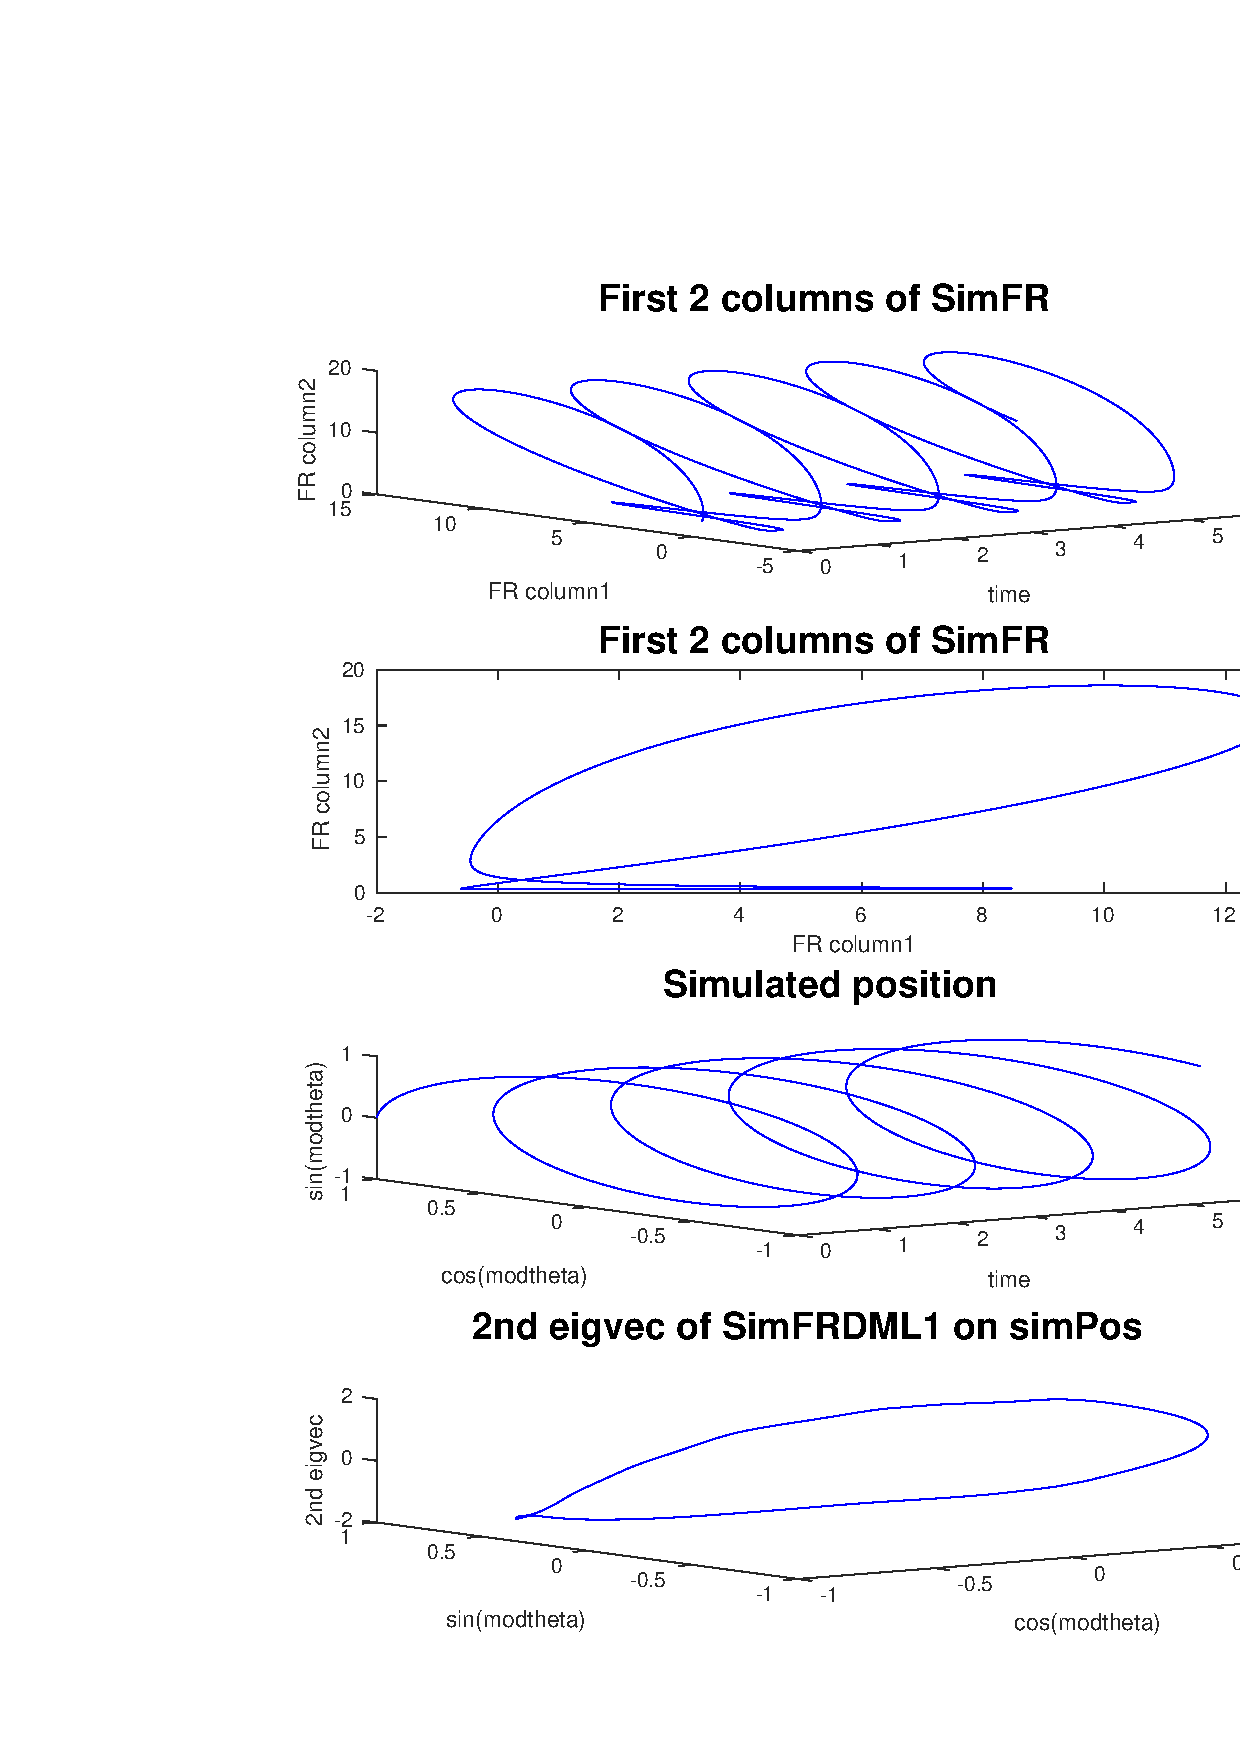
\includegraphics[width=\paperwidth]{/home/tesylvia/Oral_Sept_2017/images/FakeBrain-plots/DM-on-FR-L1.pdf}}
\end{figure}



\subsubsection{PCA on simulated FR  data}

\begin{figure}[H]
  \centering
   \makebox[\textwidth]{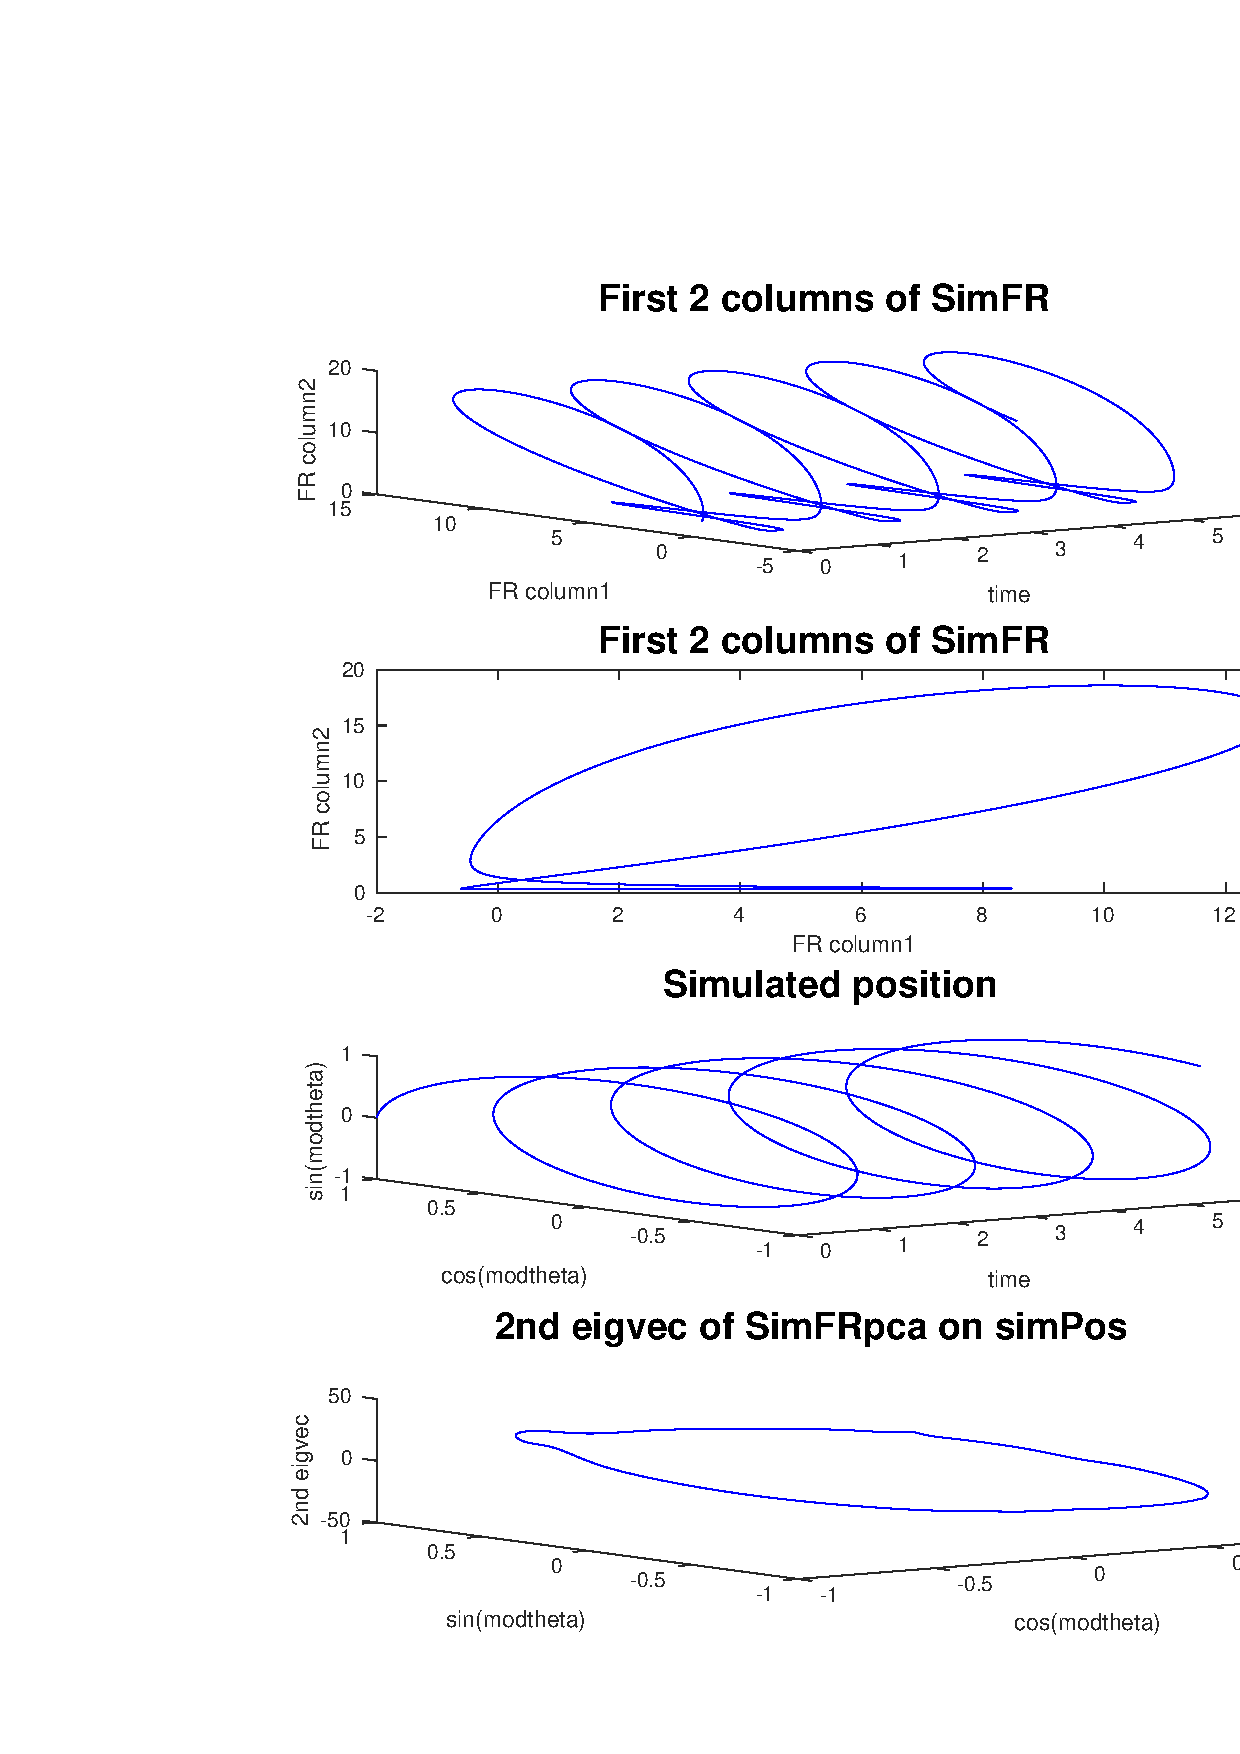
\includegraphics[width=\paperwidth]{/home/tesylvia/Oral_Sept_2017/images/FakeBrain-plots/PCA-on-FR.pdf}}
\end{figure}


\subsection{Simulation results on previous time data}
In these sections, we show our results of diffusion maps (DM),on simulated previous time (Simprevtime) using the l1 distance (SimprevtimeDML1)and  PCA on Simprevtime (SimprevtimePCA).



\subsubsection{DM on simulated prevtime data using L1 distance}

\begin{figure}[H]
  \centering
   \makebox[\textwidth]{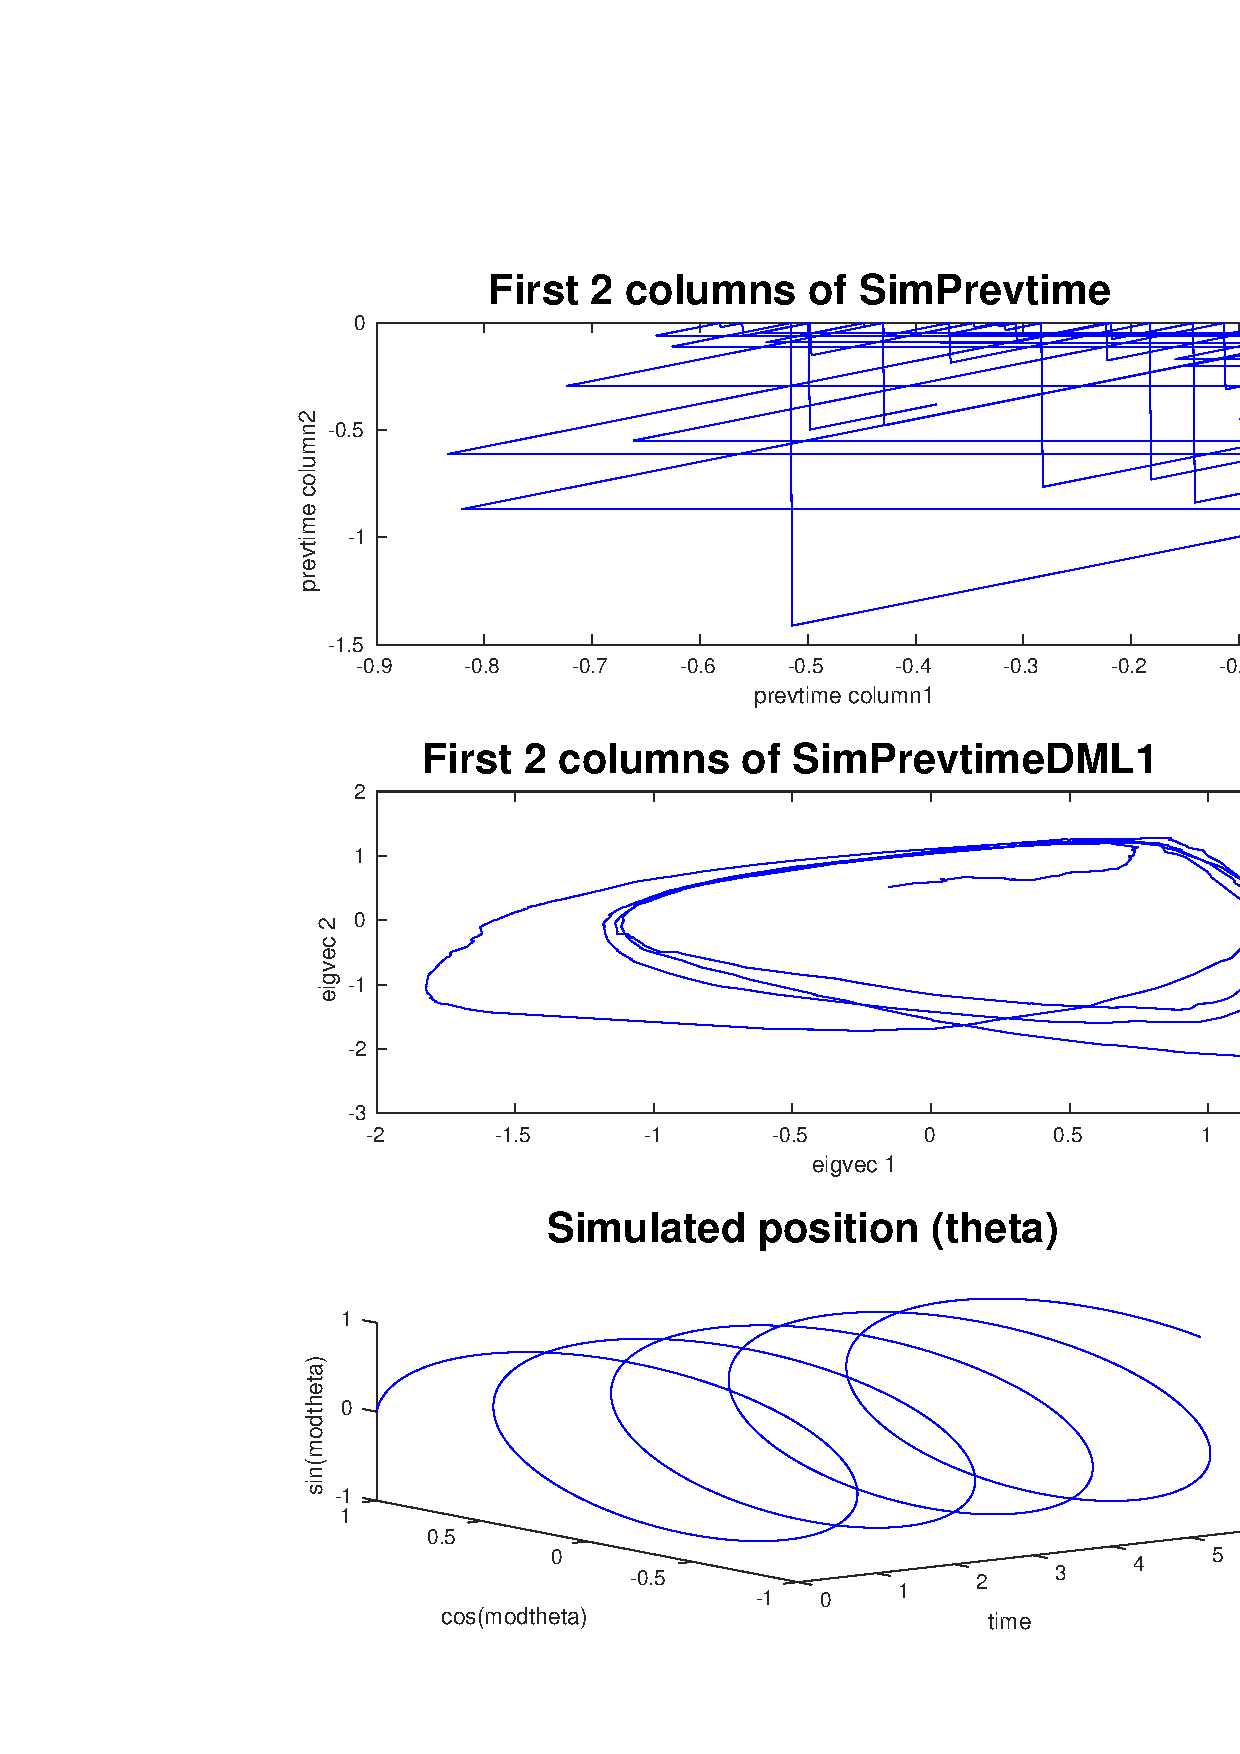
\includegraphics[width=\paperwidth]{/home/tesylvia/Oral_Sept_2017/images/FakeBrain-plots/FirstL1DM.pdf}}
\end{figure}



\begin{figure}[H]
  \centering
   \makebox[\textwidth]{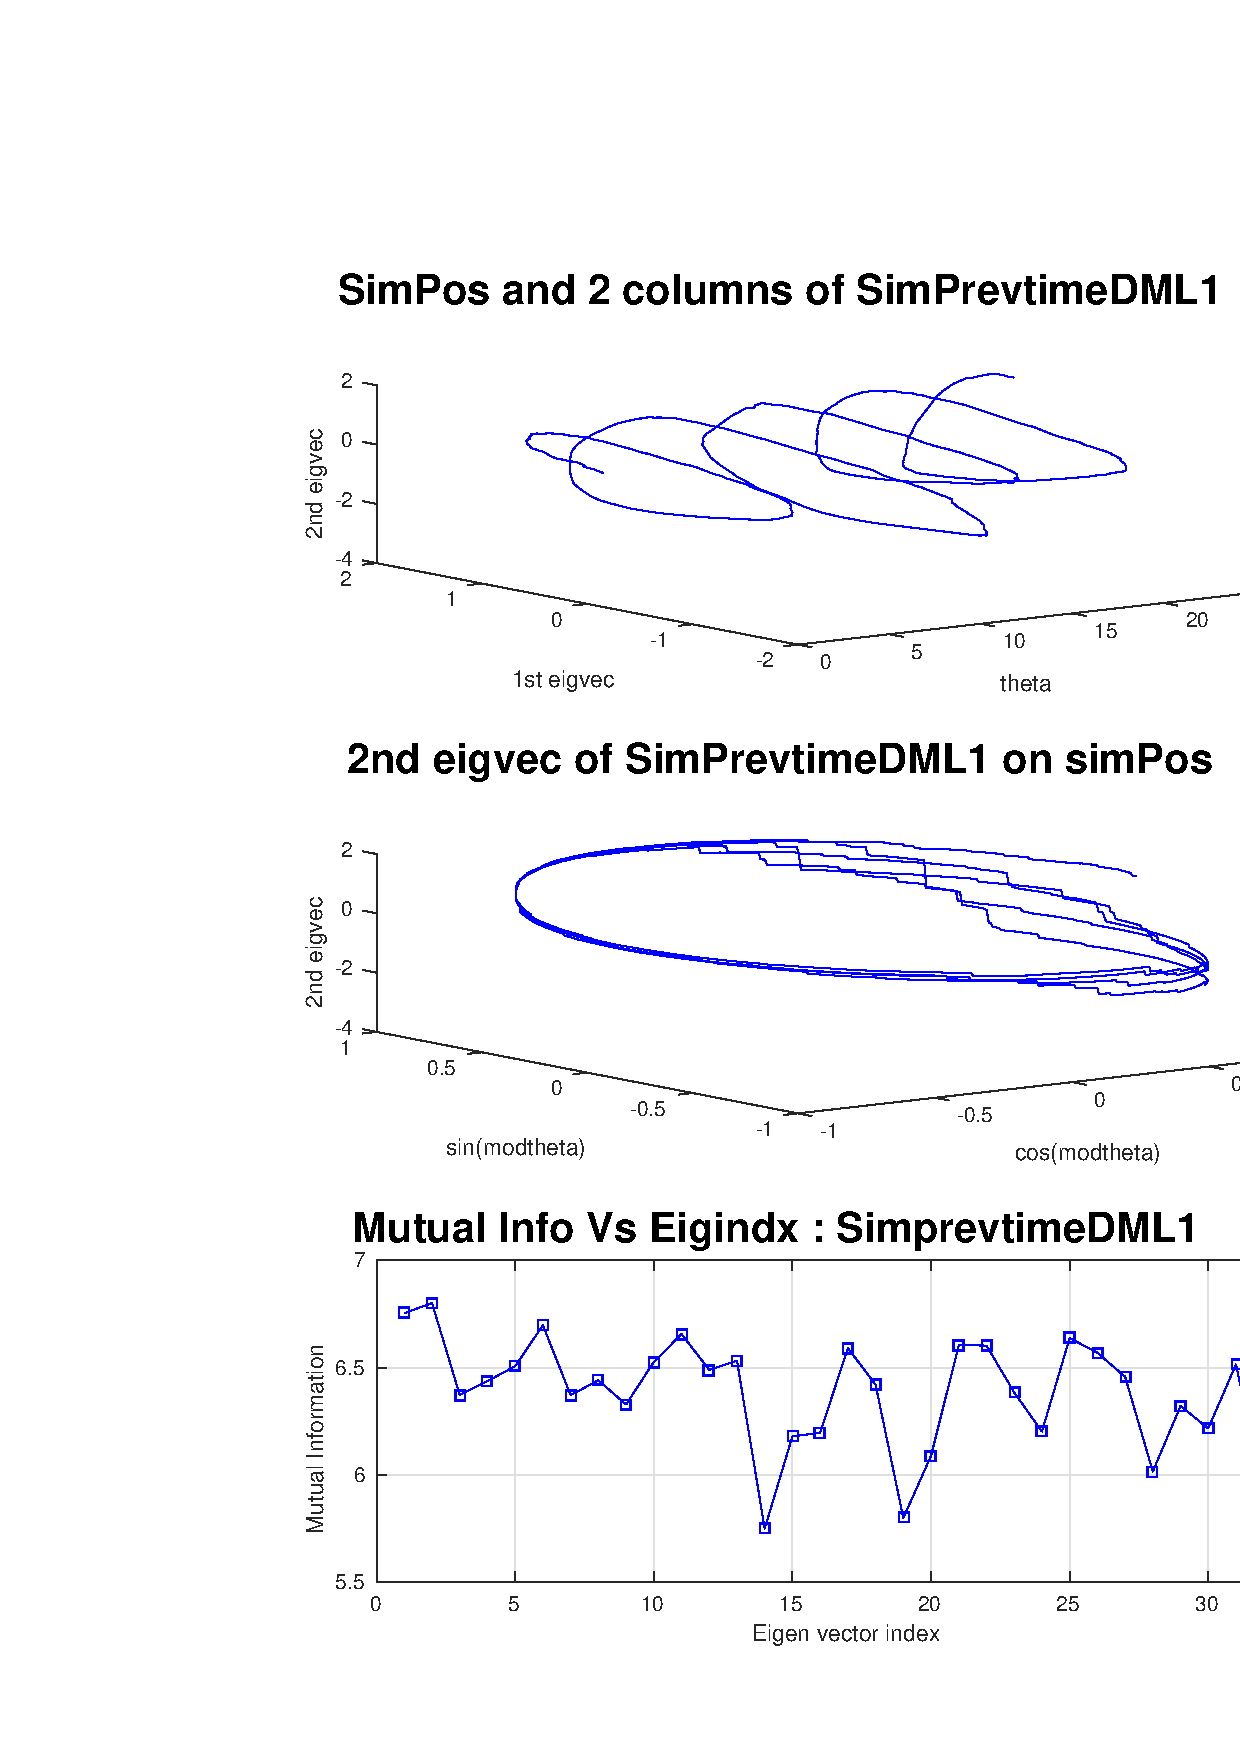
\includegraphics[width=\paperwidth]{/home/tesylvia/Oral_Sept_2017/images/FakeBrain-plots/SecondL1DM.pdf}}
\end{figure}




\subsubsection{PCA on simulated prevtime data}

\begin{figure}[H]
  \centering
   \makebox[\textwidth]{\includegraphics[width=\paperwidth]{/home/tesylvia/Oral_Sept_2017/images/FakeBrain-plots/FirstPCAMI.pdf}}
\end{figure}



\begin{figure}[H]
  \centering
   \makebox[\textwidth]{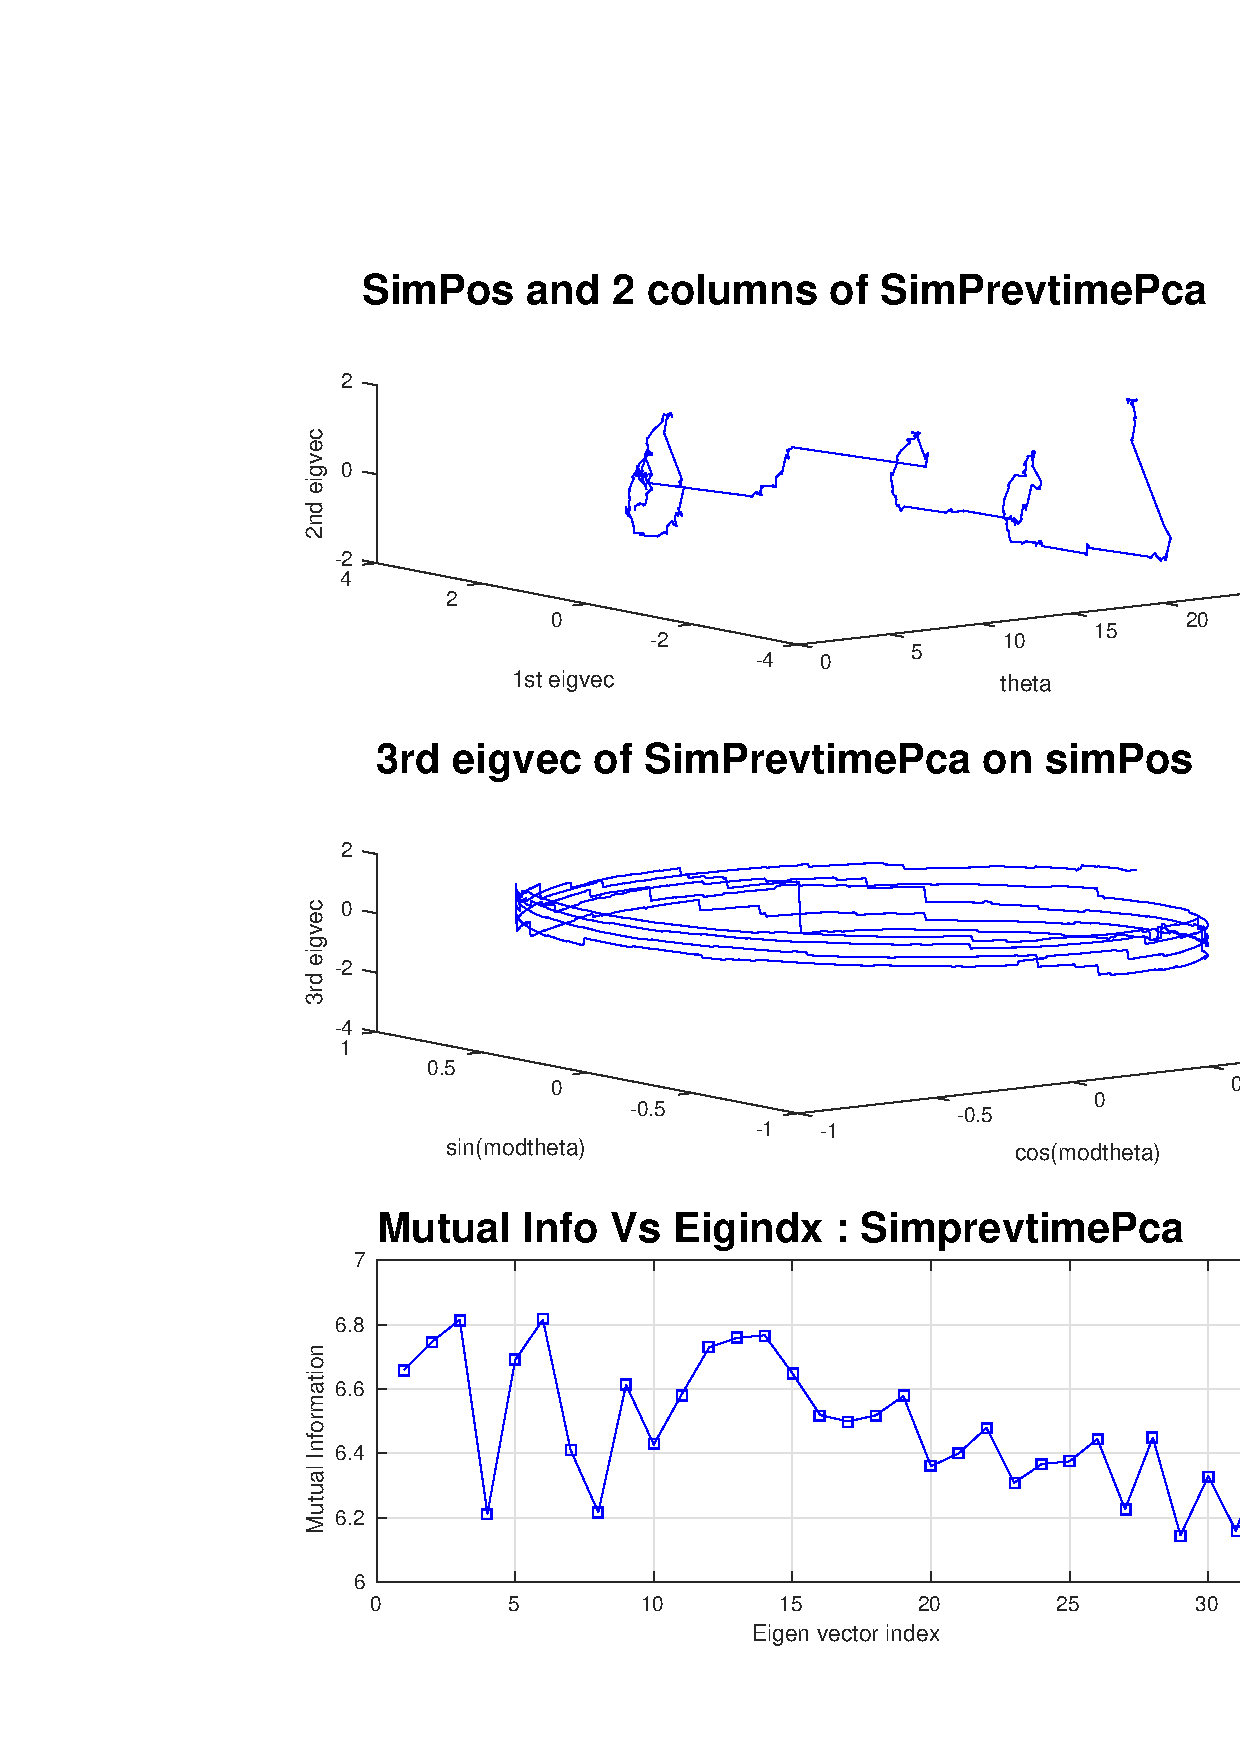
\includegraphics[width=\paperwidth]{/home/tesylvia/Oral_Sept_2017/images/FakeBrain-plots/MI-2PCA.pdf}}
\end{figure}




































































%\begin{itemize}
%\item show the graphs/results package
%\item this is how we're interpreting the results
%\item why does this matter?
%\item what measure of goodness did you use?
%(Fisher Vs Shannon information)

%%==========suggested by Duane============================================
%\item Mention that there are other ways of checking measures of goodness
% e.g the one provided by diffusion maps, Bayesian decoding refer to the nature
% and review artcicle.


%\end{itemize}










%\mychapter{7}{Discussion}
\section{Discussion/interpretation}
In this section, first, we explain our observations based on our experimental
results on synthetic and real-world data. We also justify our use of the l$_{1}$ norm for our distance measure.
Finally, we discuss the strengths our model and suggest possible future directions of addressing some short comings of our model.


\subsection{Interpretation of our results}
Analyzing synthetic data using previous time vectors produces a wide variety of geometric differences, as compared to  using firing rate vectors, as is typical.
While the differences are prominent, as revealed in the preceding plots, their 
statistical significance is as yet unknown. We regard this observation as a potentially exciting area for future investigation and believe it is worthwhile 
to highlight several of the salient differences.\\

For instance, in figure (), the output based on previous time shows that 
the animal made about four laps around the  simulated track. This is not visible while using the firing rate.\\

In addition, variability is apparent along the different trajectories taken by the animal around the track while using previous time data, whereas data based on the firing rate shows no such variability. The variability revealed by previous time data is an exciting area for future investigation.\\

Synthetic results based on using the l$_{1}$ distance in the diffusion maps algorithm appear to yield a perfect reconstruction of the simulated position of the animal compared to that using PCA. \\

On the real-world results, we see that the portion of the circular truck reconstructed by the diffusion maps algorithm on previous time data is larger than that returned by PCA, which further emphasizes the exciting nature of our approach.\\

Finally, both the diffusion maps algorithm and PCA are unable to reconstruct the real-world circular truck based on firing rate data which shows that our approach of preprocessing data by looking the time since the previous spike, may be a possible worthwhile approach to analyzing spike train data from the rat hippocampus.

\subsection{Strengths of our approach}
First, preprocessing spike train data by forming new previous time vectors and using the diffusion maps algorithm with an appropriate metric provides a low dimensional model for the data which is independent of the labels of the neurons nor the positions of the place fields in space. 
Second, since only a very small subpopulation of neurons is active at a particular moment, there is often a lot of missing information in the firing rate data provided by the experimentalist.
In particular, this phenomenon corresponds to having gaps between 
neighboring place fields within our simulated place field model. Nevertheless, sampling data from the previous time function provides information about neural activity even when a large portion of the neural population is inactive. 

(To Duane: it looks like the point below negates what I just wrote above.
Should I delete it?)
In addition, using the diffusion maps algorithm does not require a dense sampling
of the neural space like other non-linear methods do, such as Laplacian eigen maps.

\subsection{Future directions}
First, at the beginning of the experiment, there are no recorded spike times.
However, we require that there is atleast one spike before a given brain state,
in order to have the previous time function defined for all time.
This raises a problem on how to address the boundary condition at the beginning
of the experiment. As it stands, we have addressed this problem by first running the experiment once to obtain the mean of the sampled previous time data, and afterwords, we insert a spike before the beginning of the experiment based on the computed previous time average, and then we recompute the new the previous time data. We think that this is not the best approach for instance in the case where the mean of underlying distribution is not defined. In addition, computing the previous time vectors twice increases the computational complexity of our algorithm. We plan to find another way of addressing the boundary condition
for the previous time vectors. For example, we plan to insert a spike before the beginning of the experiment based on samples drawn from a correctly estimated underlying model of the data.\\

Second, we currently do not have a measure of error for analysing the  effectiveness of our approach. One possible confound in the plots is that the high  mutual information may be to due space noise, such as the animals head directions while running along the truck. This opens a variety of possible interpretations of the data. We plan to use the Fisher information as a goodness of measure in future work. We think that the Fisher information is a likely a good measure of error, since it imposes a continuity assumption on the underlying model and is highest when then the variance of the estimated model parameter is very small.
This should help to yield a more reliable estimate of the animal's position along the truck. \\

In addition, non-linear methods like diffusion maps do not yield an explicit function between the input and output space. This provides a challenge on how to evaluate the performance of the algorithm. Current approaches first add a new column to the original data set and then recompute the embedding on order to obtain a prediction of the new point in the embedded space. However, diffusion maps runs out of memory for large data sets since it requires computation of a full $n \times n$ matrix given n data points. This makes it difficult to use out-of-sample extensions as a goodness of measure in large scale neural recordings.\\

Third, in our current approach, we do not have an explicit model which enables
us to see how the system evolves over time.
Our results are independent of the precise time at which the spikes occur since the position of the animal is encoded by vectors corresponding to brain states
sampled uniformly at random. Thus we are unable us to quantify the impact of precise spike timing on decoding the underlying stimuli such as the position
of the animal on the truck. We aim to design a model which takes into account the precise timing of the spikes. 

Finally, we plan to look at other types of distance measures for quantifying neural response variability such as variants of the kendal tau distance 
or a weighted combination of some existing distances. We have used the l$_1$
norm instead of the l$_{2}$ norm because the latter emphasizes large differences between data points which diverges from our goal of learning similar brain states 
based on pairwise distances between spike trains.


An improved approach such as the one we envision and outline here 
may lead to new theories of mathematical neuroscience for analysing spike train data from animal hippocampuses.















%Our first step was to determine what dimensionality reduction algorithms to use.
%We decided to use Laplacian eigmaps \cite{belkin2003laplacian} and Diffusion Maps \cite{coifman2006} which are both non-linear dimensionality reduction algorithms.
%why?----to be addressed later.
%Initially, we smoothed the spike data using an exponential kernel defined by
%
%\[
%  K_{\tau}(t) =
%  \begin{cases}
%                 \frac{1}{\tau} \exp(-\frac{t}{\tau}) & \text{if $t > 0$} \\
%                  0 & \text{elsewhere} 
%  \end{cases}
%\]
%
%\subsection{Observations}
%We found that using Laplacian eigen maps to get an embedding based on the firing rate tried to
%recovered the position of the rat but could not reflect any variations along the path
%e.g the animal could have looked away from the track or run in a ragged fashion around the track.\\
%
%We also found that whenever there were gaps between the receptive fields (cases with no spikes),Laplacian Eigen Maps (LAM) performed poorly.
%This is because the nearest neighbor graph (based on the Euclidean distance used in (LAM) yields several connected components (i.e, the graph is disconnected).
%Since the eigen value decomposition step  in LAM is only applied on the largest connected
%component of the graph, the eigen vectors output by LAM are shorter than the total number of original data points (spike times). Thus the embedding provided by LAM is in accurate in some
%instances due to the "coverage" problem.\\
%
%Diffusion Maps (DM) algorithm tends to run out of memory in case of large instances
%so we were unable to compare the performance of both LAM and DM when using the firing rate.
%This is not true: First redo the analysis on sonet since you need to show that
%previous/next time is an improvement over the traditional firing rate.
%
%\subsection{Remedy for the coverage problem}
%Inspired by David Redish's idea, we decided to create previous and next time vectors which
%give us information even when there is no spike.
%This is the direction which seems promising at the moment since it tends to over come
%the problem of coverage. what is the coverage problem? (see reference on tunning curves).
%We then used the exponential kernel as our metric on the previous and next time data
%to generate a distance metric which is the main input in Diffusion Maps algorithm.
%
%
%
%



\mychapter{8}{Future work}


%%%%%%%%%%%%%%%% Generate a Bibliography%%%%%%%%%%%%%%%%%%%%%%%%%%%%%%%%%%%%%%%%
%%==== put the bibliography after all sections=====
% but above end document===========================
\pagebreak

%add a bibliography using mendeley

\bibliography{/home/tesylvia/Oral_Sept_2017/References/library.bib}

\bibliographystyle{unsrt}




\end{document}
